\documentclass[12pt, a4papre]{article}
\usepackage[catalan]{babel}
\usepackage[unicode]{hyperref}
\usepackage{amsmath}
\usepackage{amssymb}
\usepackage{amsthm}
\usepackage{xifthen}
\usepackage{listings}
\usepackage{float}
\usepackage{siunitx}
\usepackage{graphicx}
\usepackage{indentfirst}

\newcommand{\norm}[1]{\lvert #1 \rvert}
\graphicspath{ {./Images/Memoria4/} }

\hypersetup{
    colorlinks = true,
    linkcolor = blue
}

\renewcommand{\figurename}{Fig.}

\author{Daniel Vilardell}
\title{Memoria Practica 4 FISE}
\date{}

\begin{document}
	\maketitle
	
	\section{Sessió 1}
	
	\textbf{Qüestió 1:} Tenim primer una fotografia amb la senyal rebuda amb un obstacle aprop del emisor i un altre amb l'obstacle a 0.5m. Podem veure que en el de 0.5m la amplitud de la senyal rebuda es de $200mV$.

	\begin{figure}[H]
		\begin{center}
		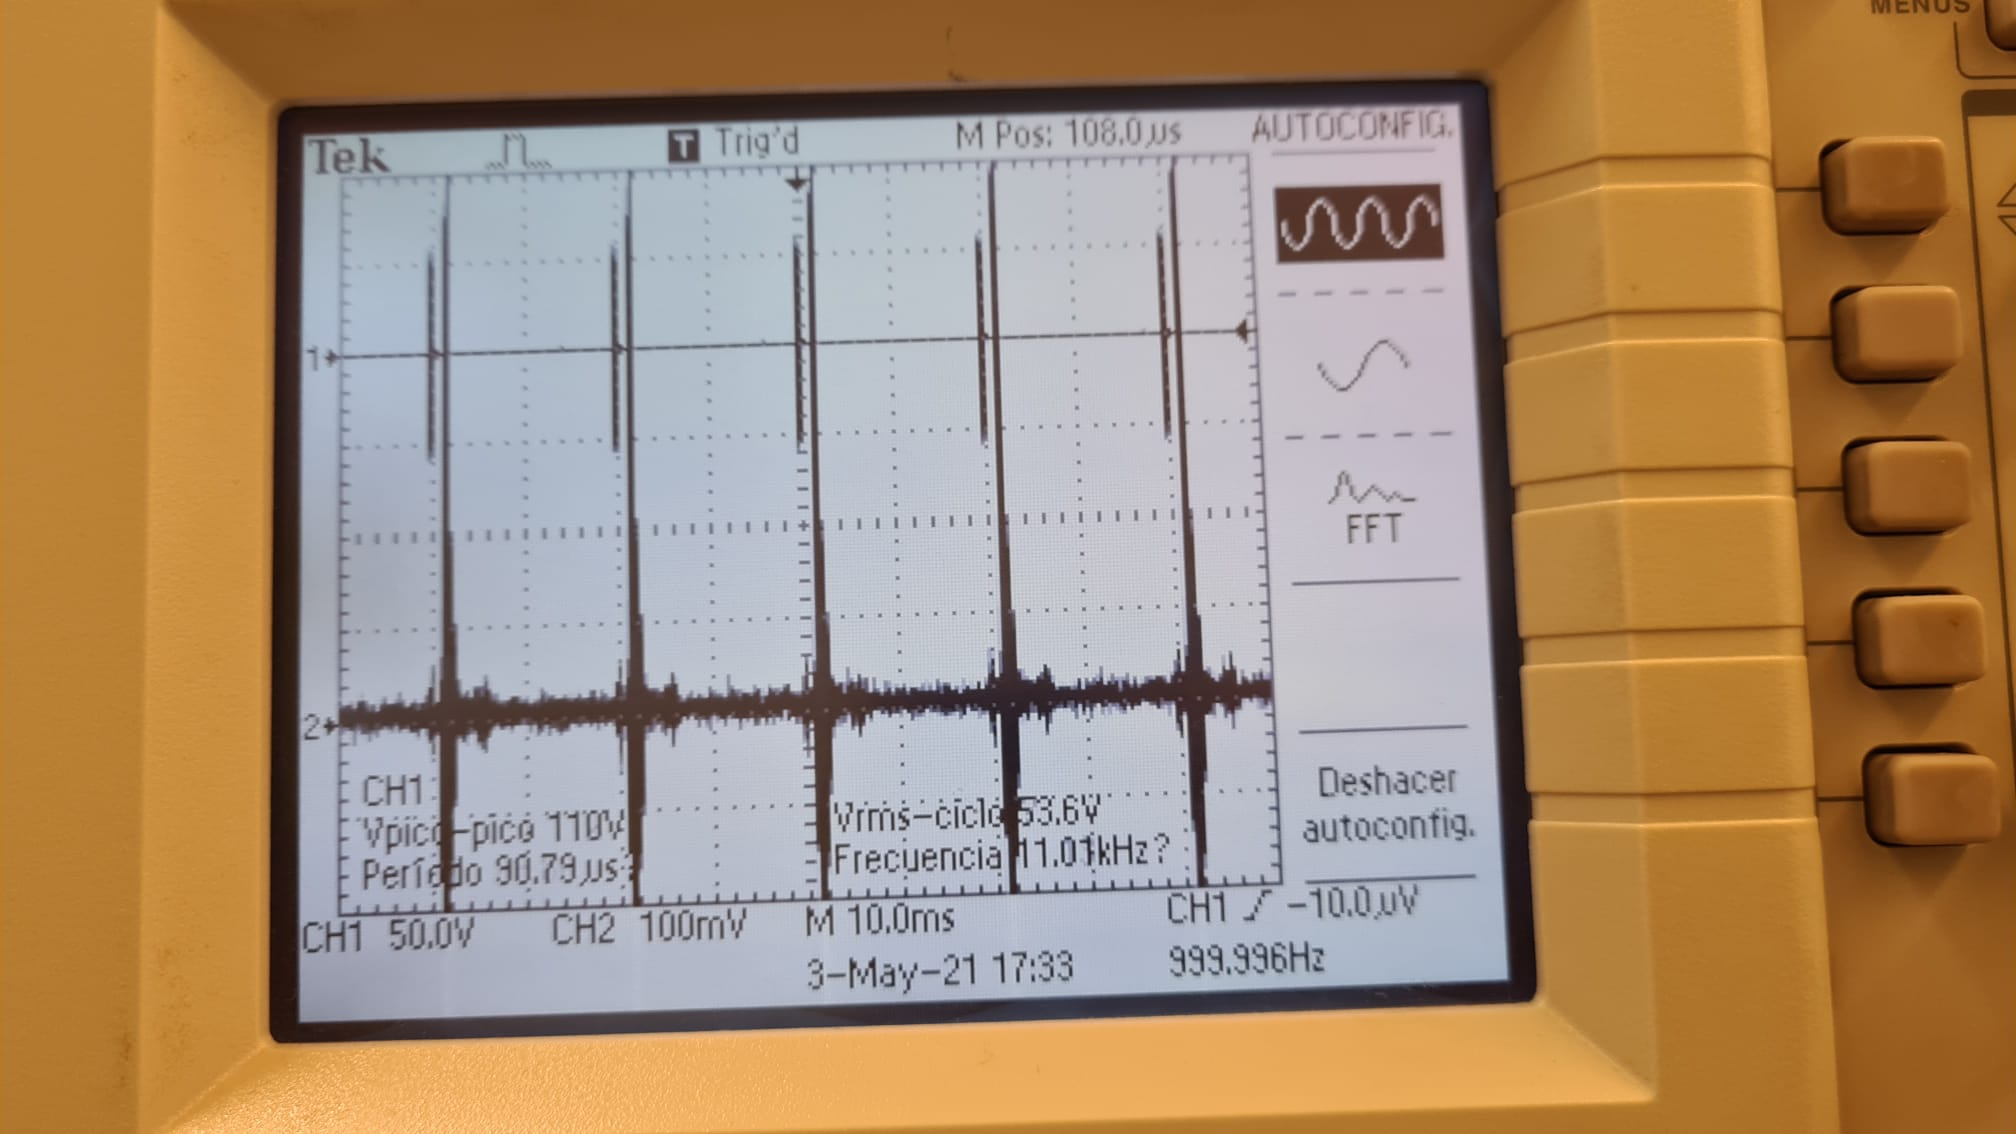
\includegraphics[width=80mm]{p4_1_1.jpeg}
		\end{center}
	\end{figure}
	
	\begin{figure}[H]
		\begin{center}
		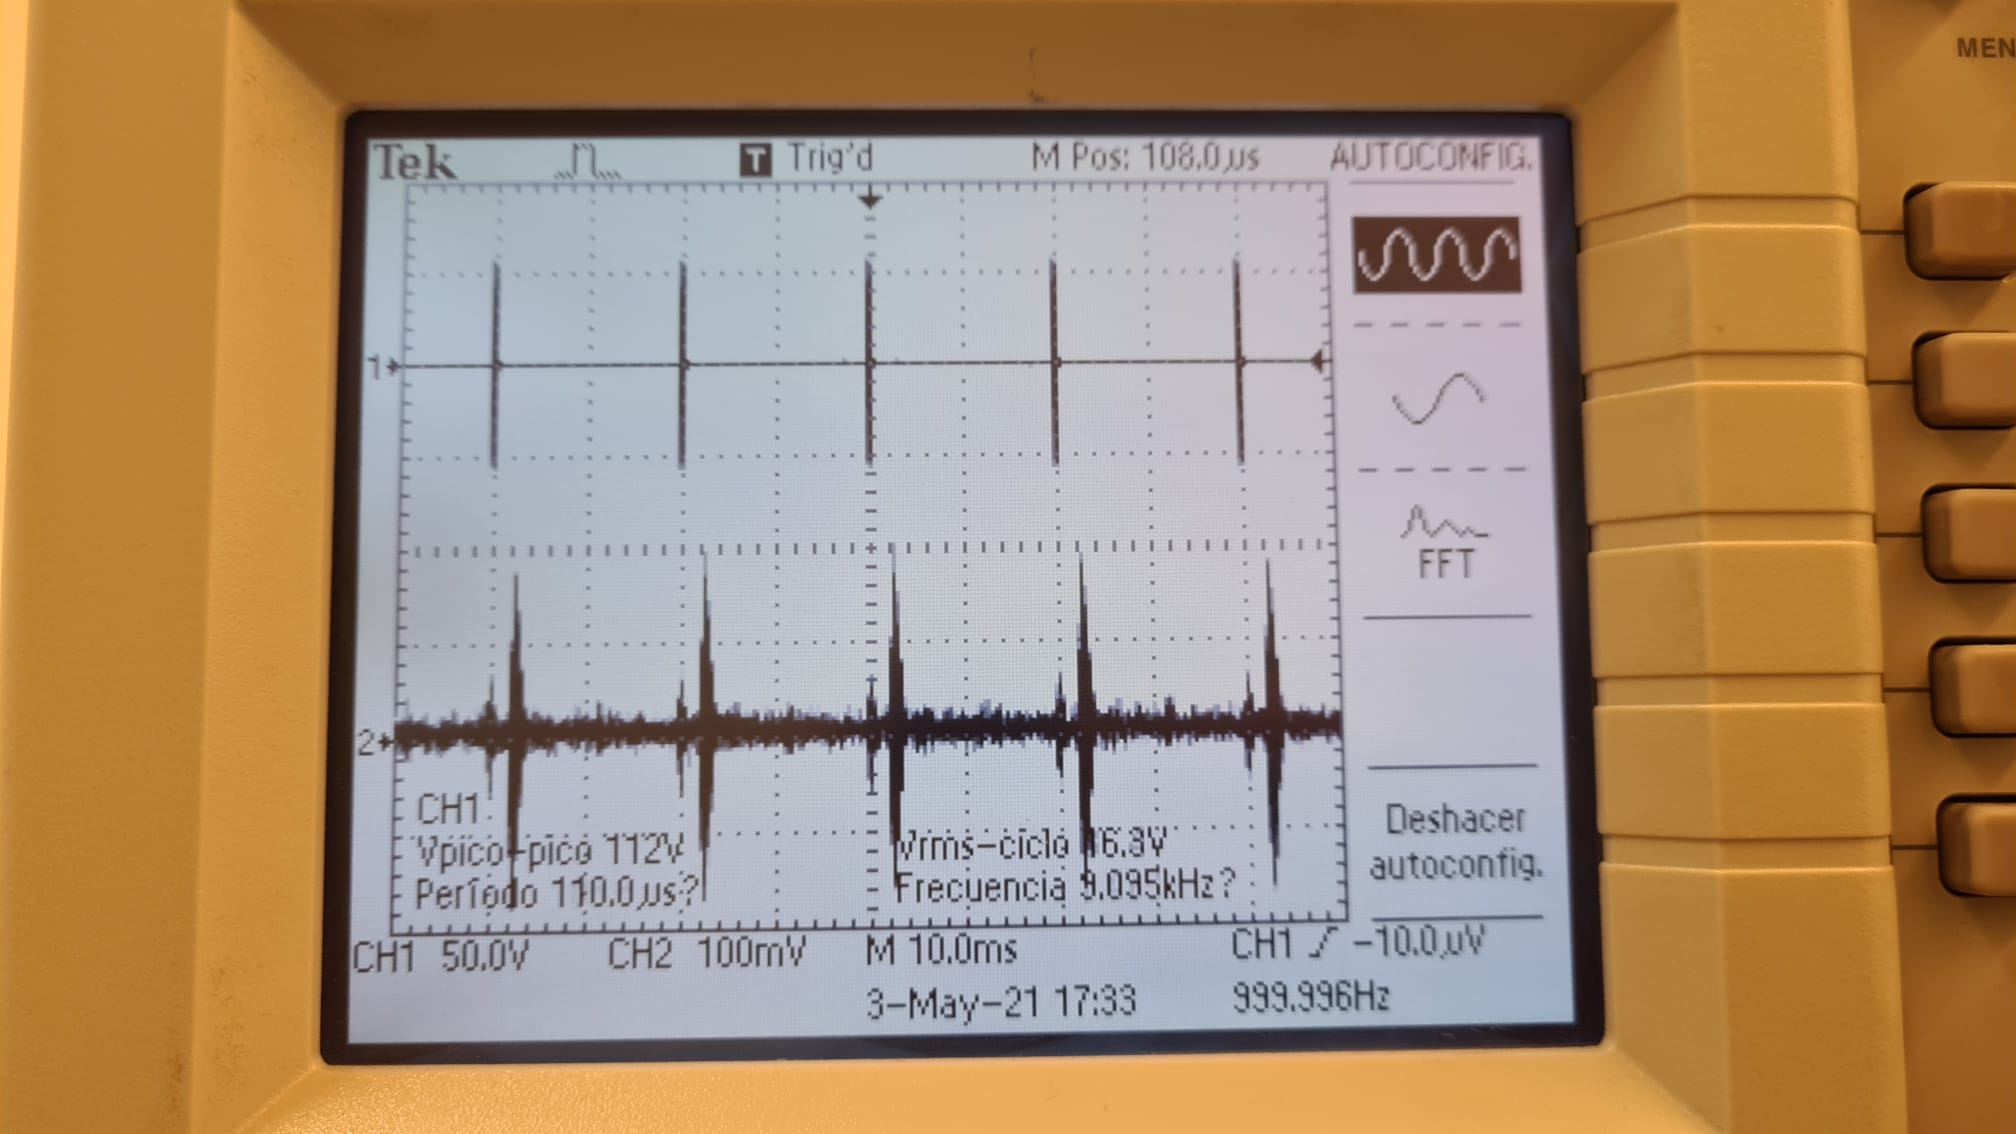
\includegraphics[width=80mm]{p4_1_2.jpeg}
		\end{center}
	\end{figure}
	
	\textbf{Qüestió 2:} El TOF es semblant al esperat i vist al estudi previ, es a dir, $2.80ms$.
	
	\begin{figure}[H]
		\begin{center}
		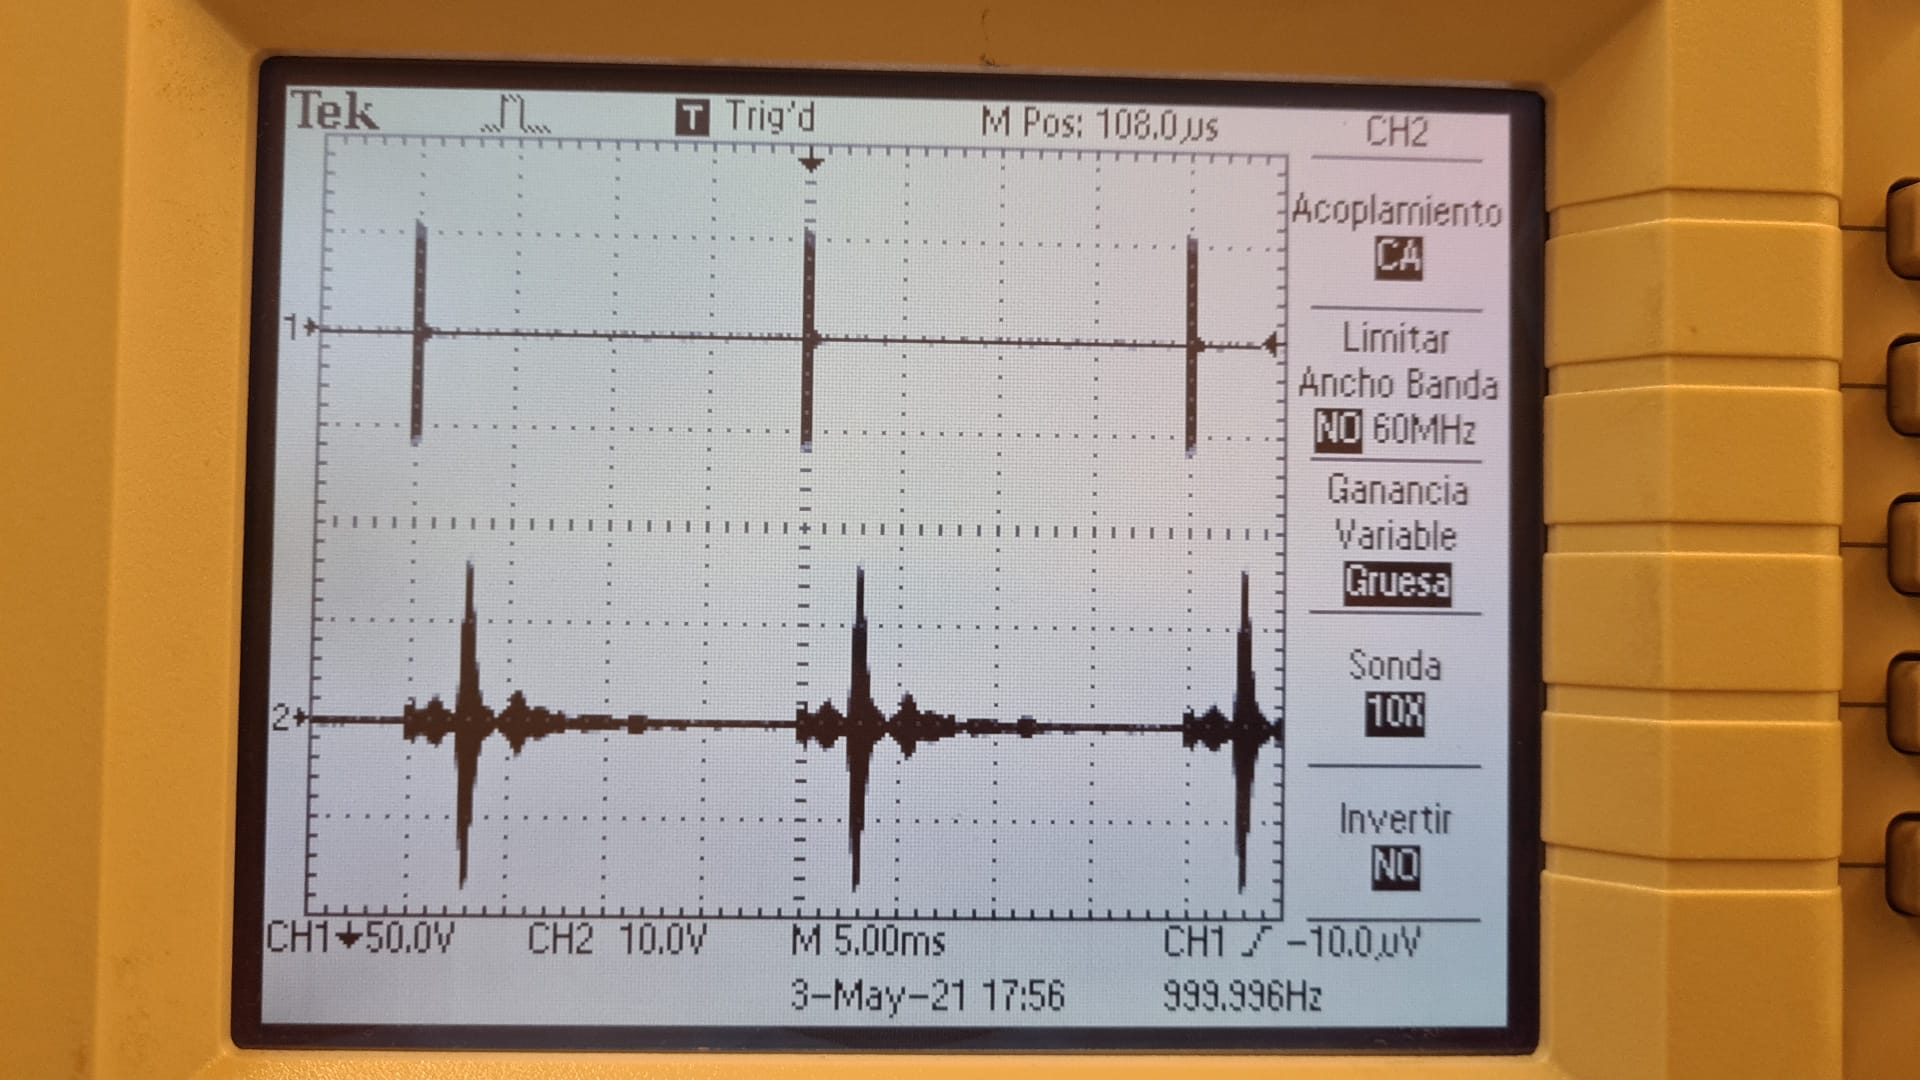
\includegraphics[width=80mm]{p4_2.jpeg}
		\end{center}
	\end{figure}
	
	\textbf{Qüestió 3 i 4:} Veiem aquí que despres de l'amplificador la amplitud es de 6V, molt superior a la que sortia del receptor. Després de posar el detector d'envolupant el resultat es el següent.
	
	\begin{figure}[H]
		\begin{center}
		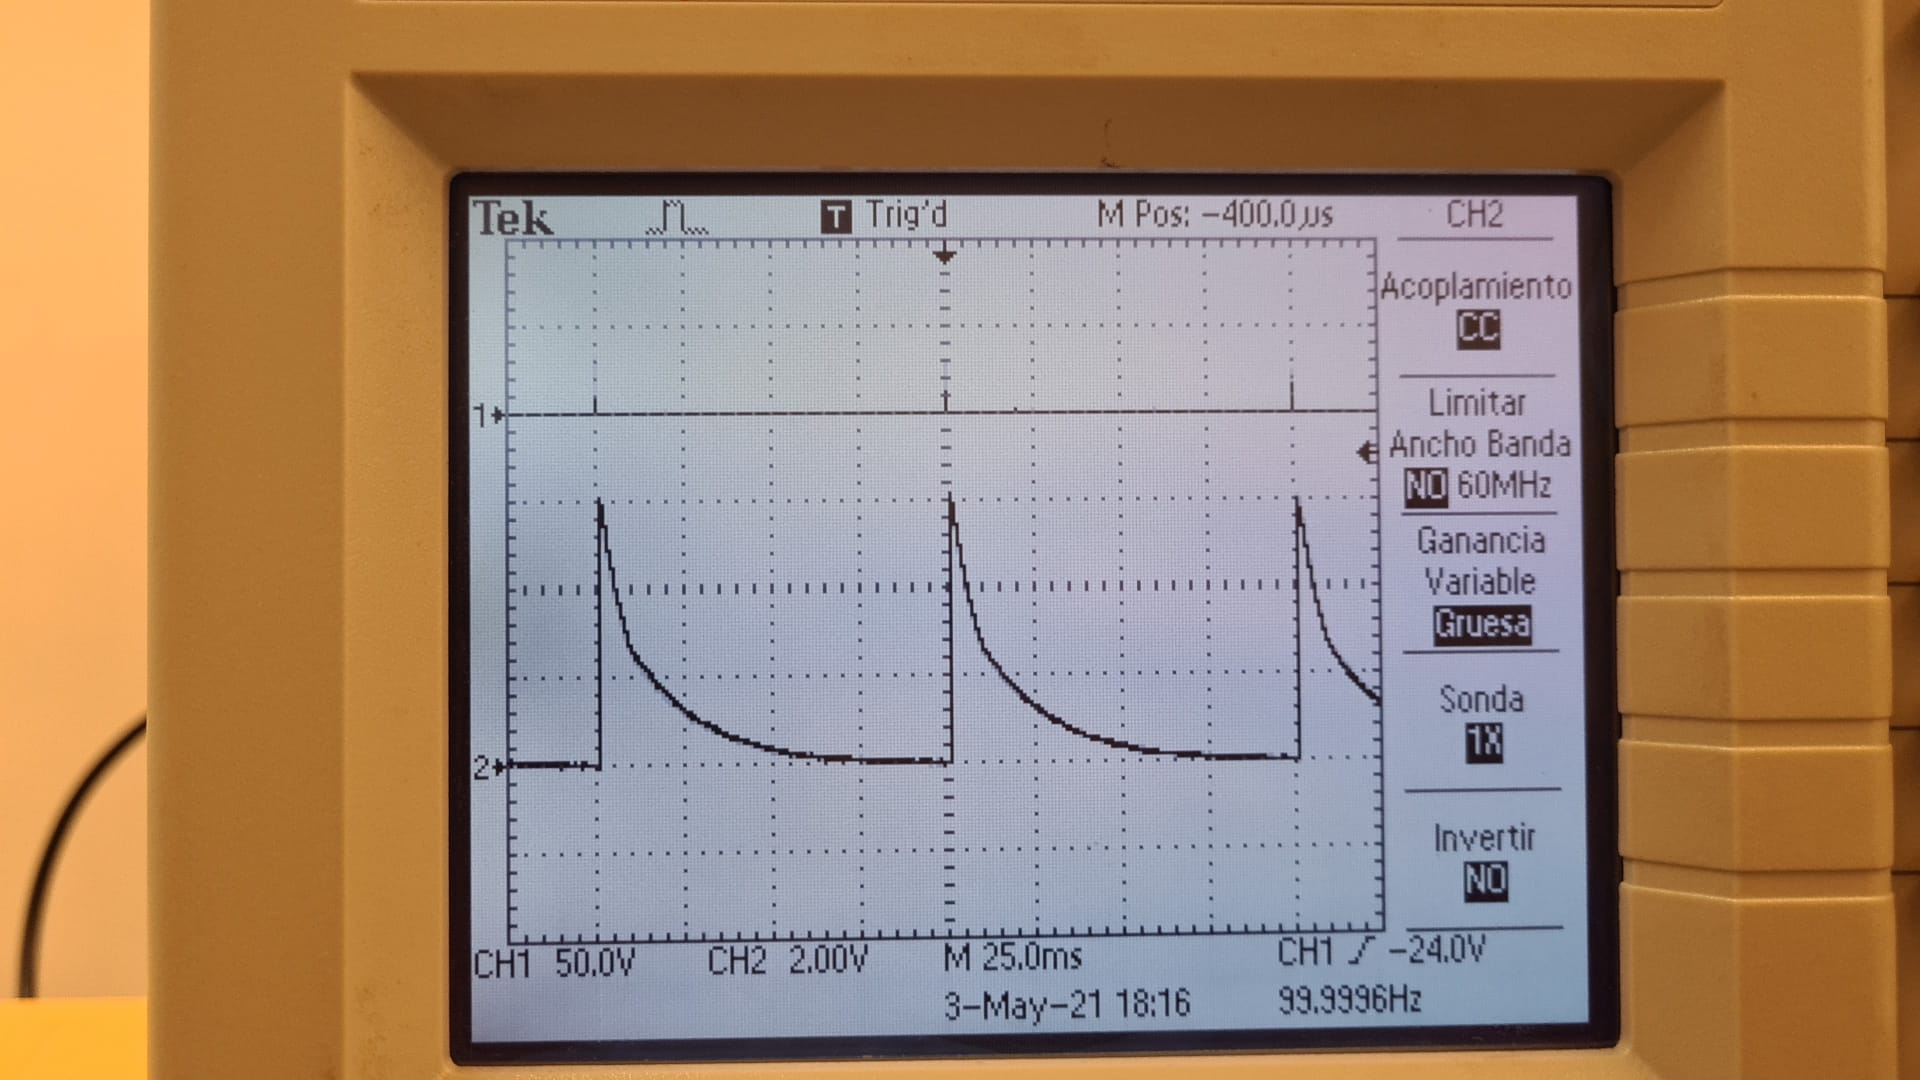
\includegraphics[width=80mm]{p_4_4.jpeg}
		\end{center}
	\end{figure}
	
	
	
	\textbf{Qüestió 5 i 6:} El resultat a la sortida per una entrada sinusoidal es la següent. Podem veure que al modificar els valors del potenciometre augmenta o disminueix la amplada del pols rectangular.
	
	\begin{figure}[H]
		\begin{center}
		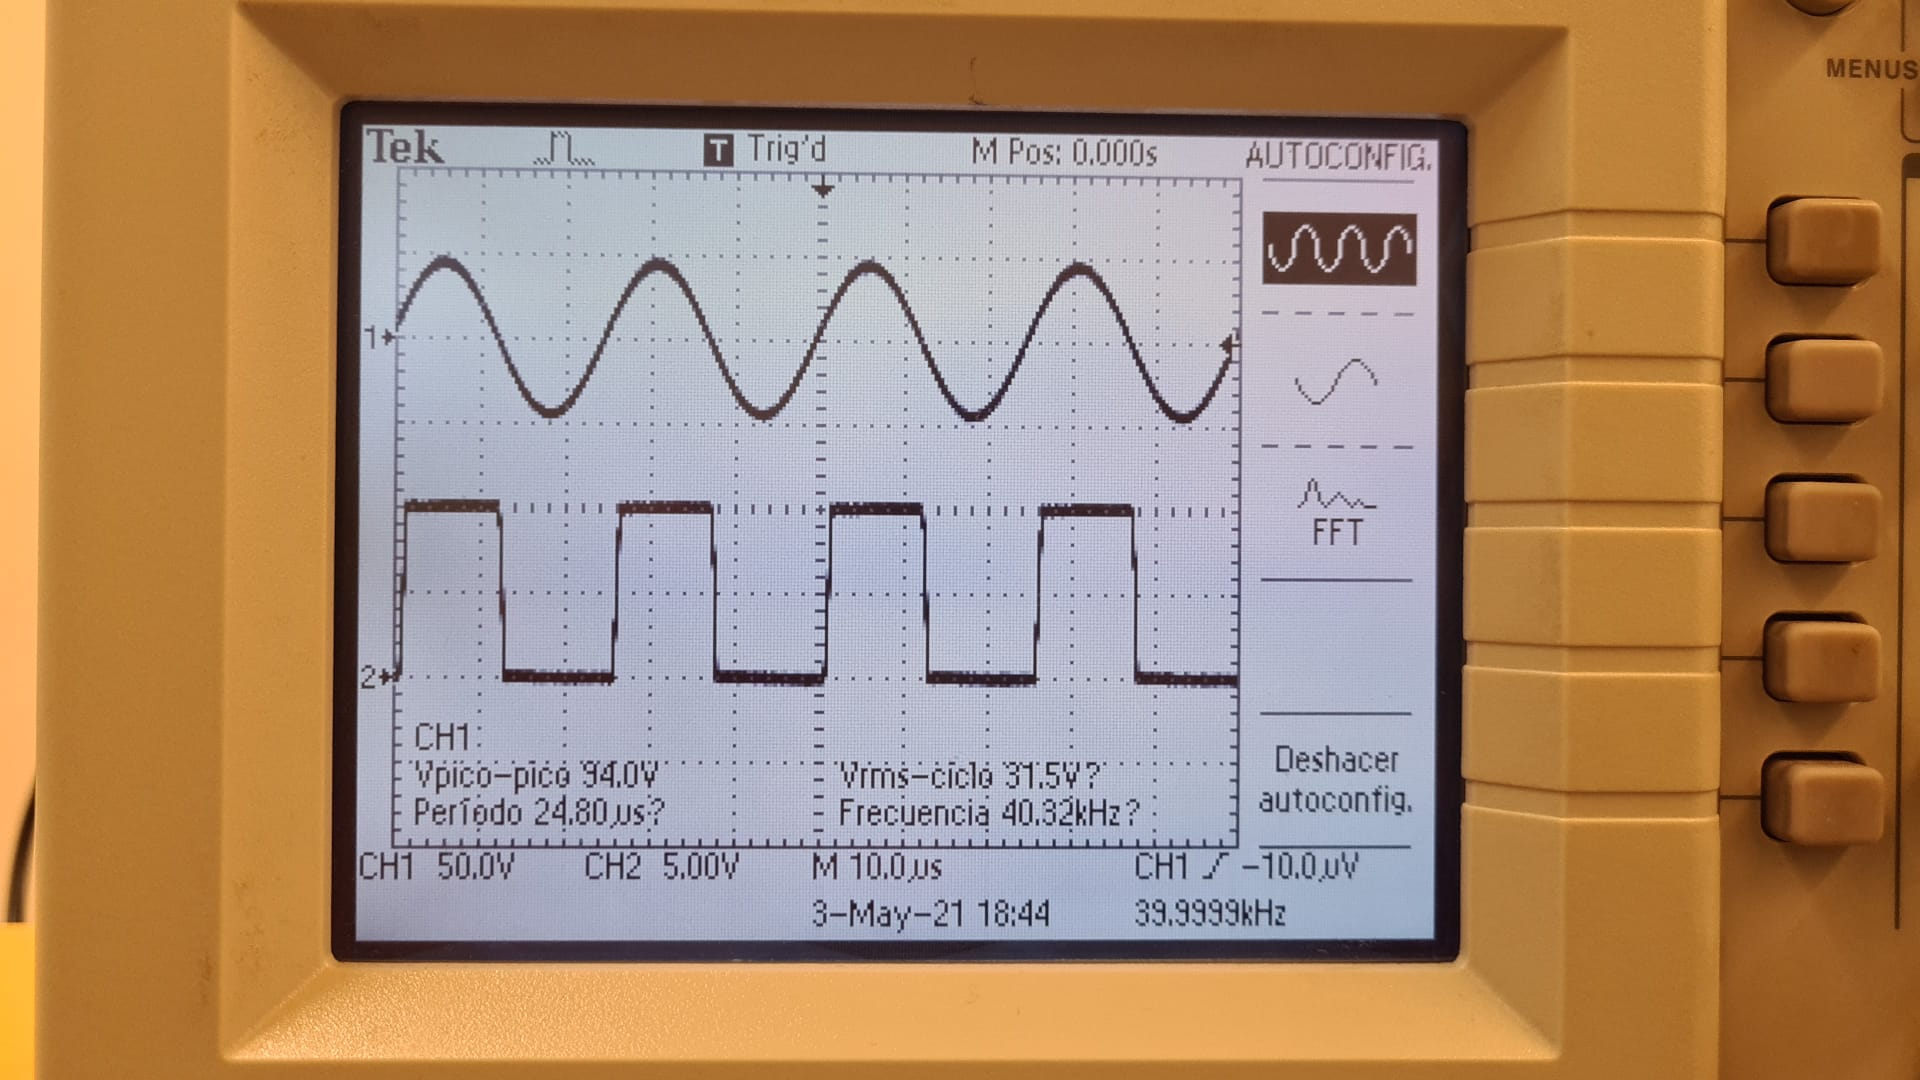
\includegraphics[width=80mm]{p4_6.jpeg}
		\end{center}
	\end{figure}
	
	\begin{figure}[H]
		\begin{center}
		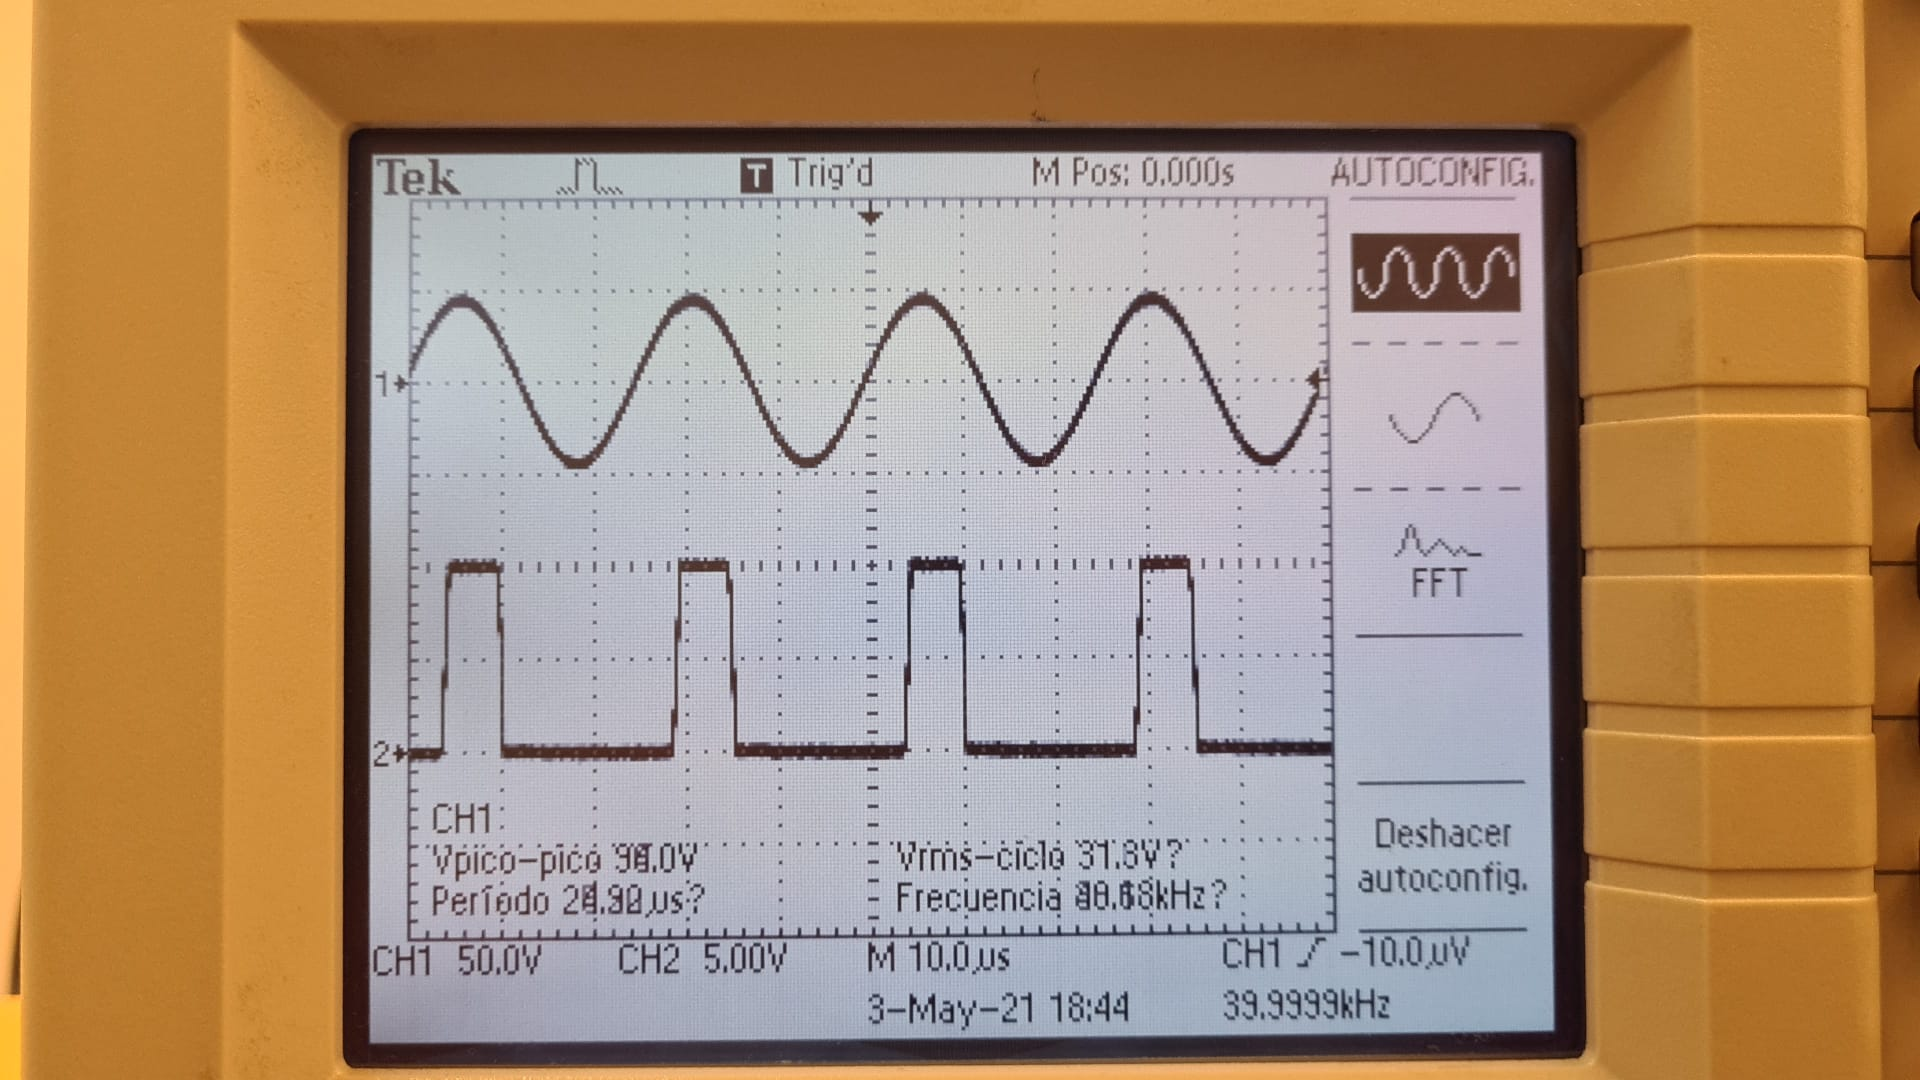
\includegraphics[width=80mm]{p4_6_2.jpeg}
		\end{center}
	\end{figure}
	
	\textbf{Qüestió 7 i 8:} Veiem que el TOF es aproximadament $2.2ms$ i per tant una distancia de $d = 340\cdot 1.1 \cdot 10^{-3} = 0.37m$. El emisor i receptor no revia res si ho posavem a mes de $0.6m$.
	
	\begin{figure}[H]
		\begin{center}
		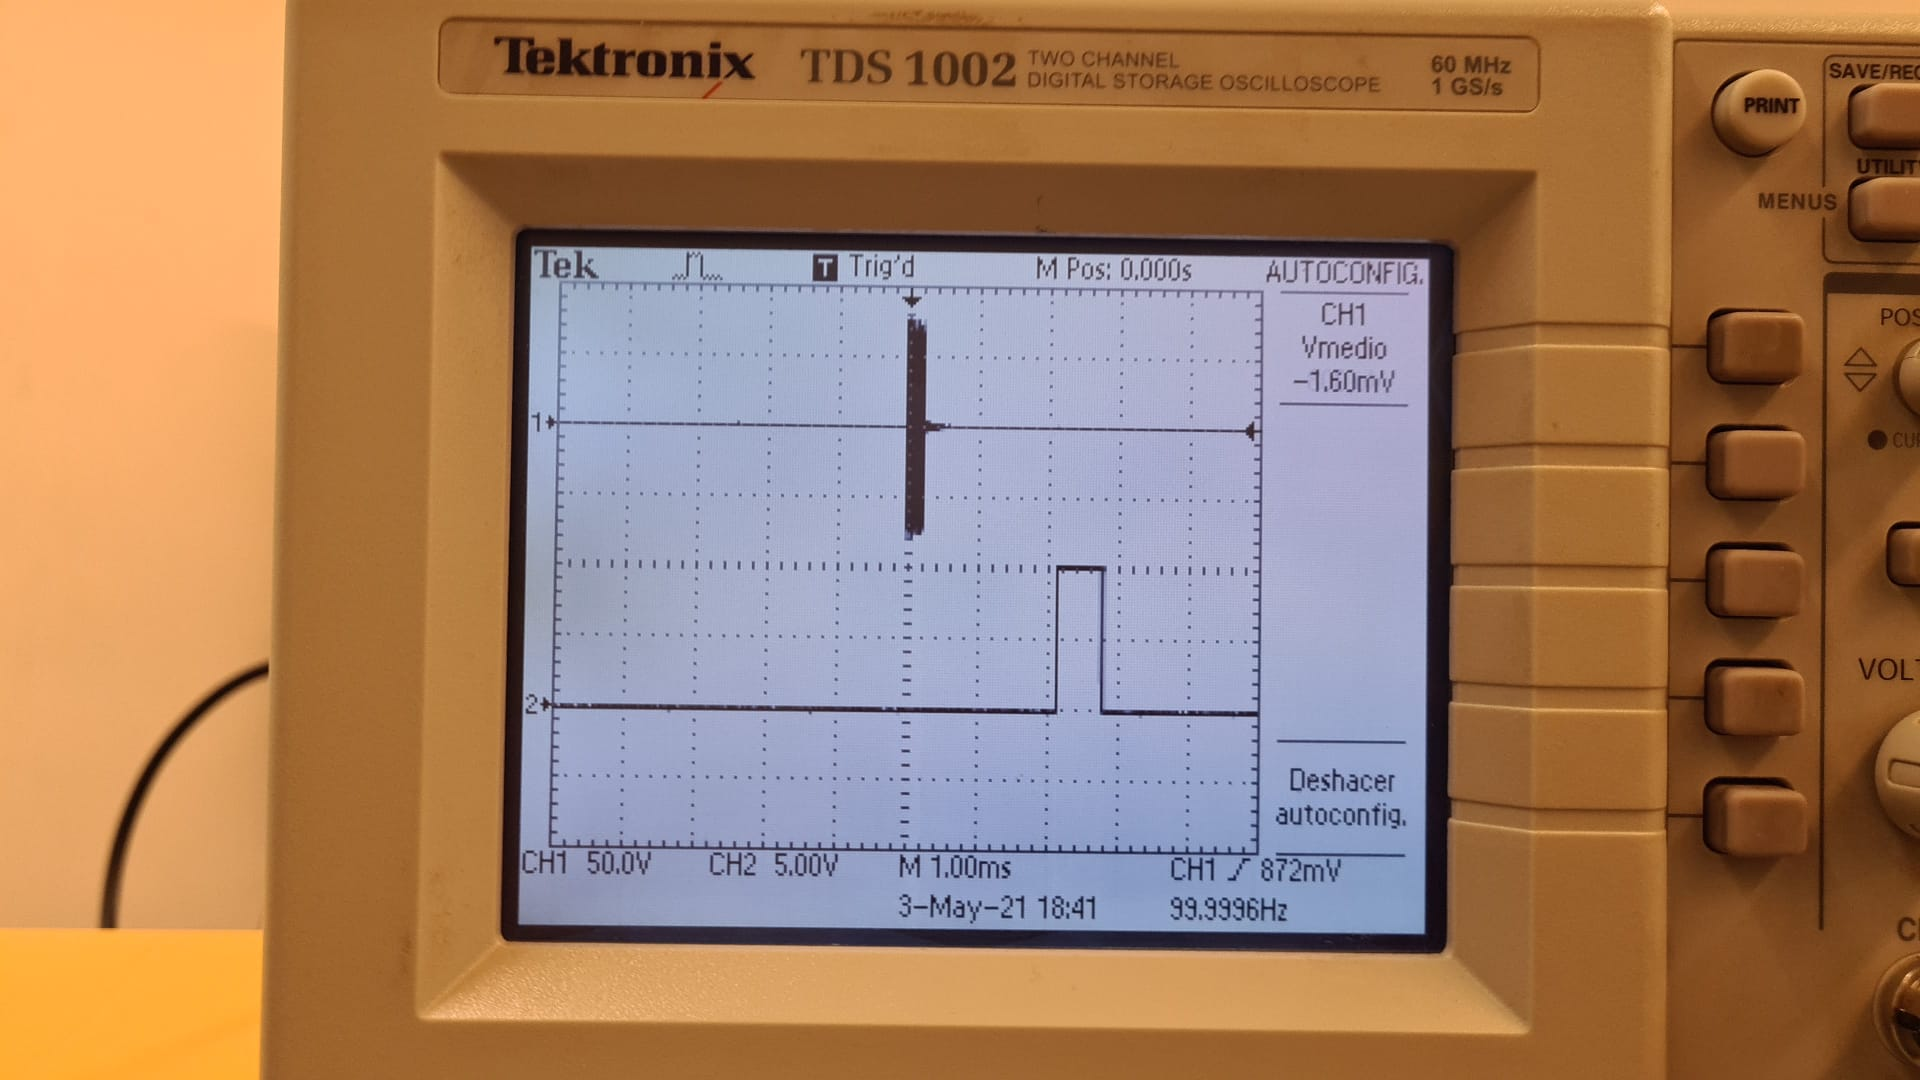
\includegraphics[width=80mm]{p4_5.jpeg}
		\end{center}
	\end{figure}
	
	\section{Sessió 2}
	
	\textbf{Qüestió 1:} Podem veure que la freqüencia maxima es de $f = 40kHz$ i la minima es de $f = 33kHz$.
	
	\begin{figure}[H]
		\begin{center}
		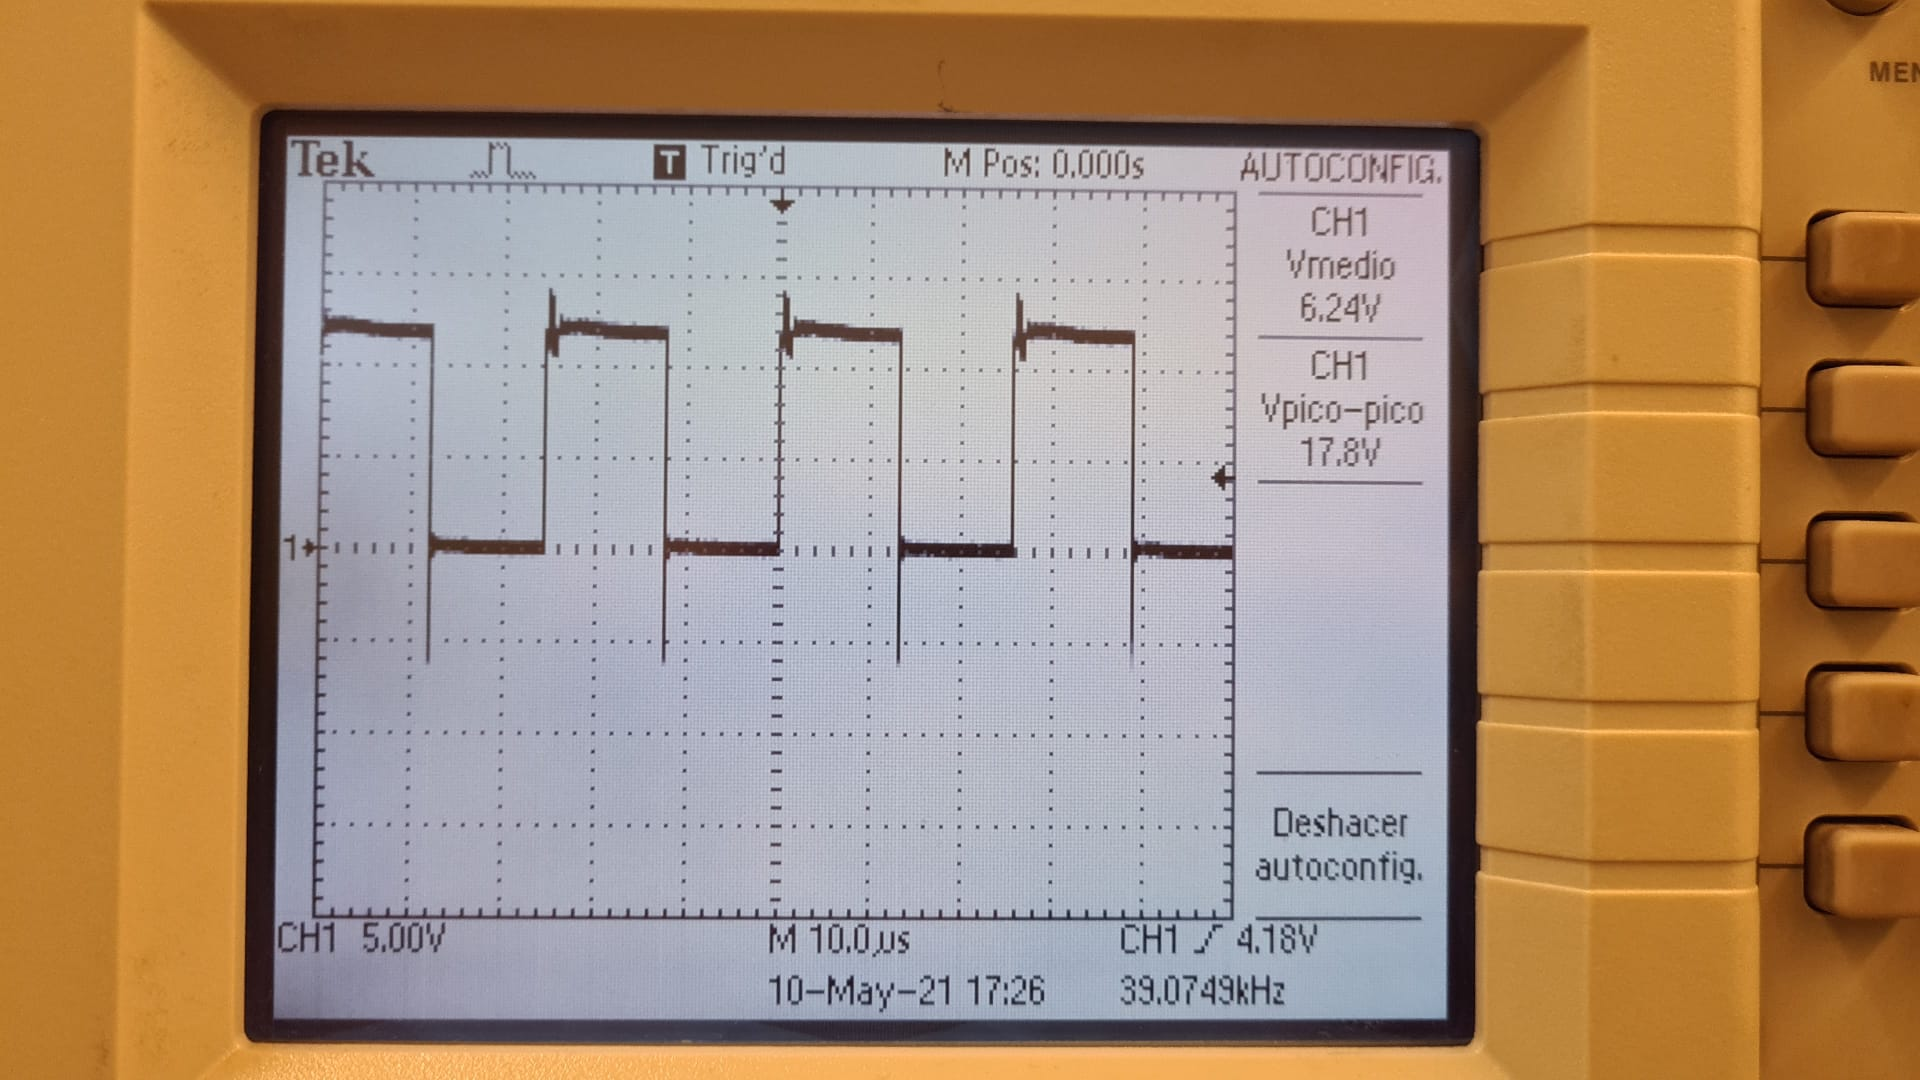
\includegraphics[width=80mm]{4_7_M.jpeg}
		\end{center}
	\end{figure}
	
	\begin{figure}[H]
		\begin{center}
		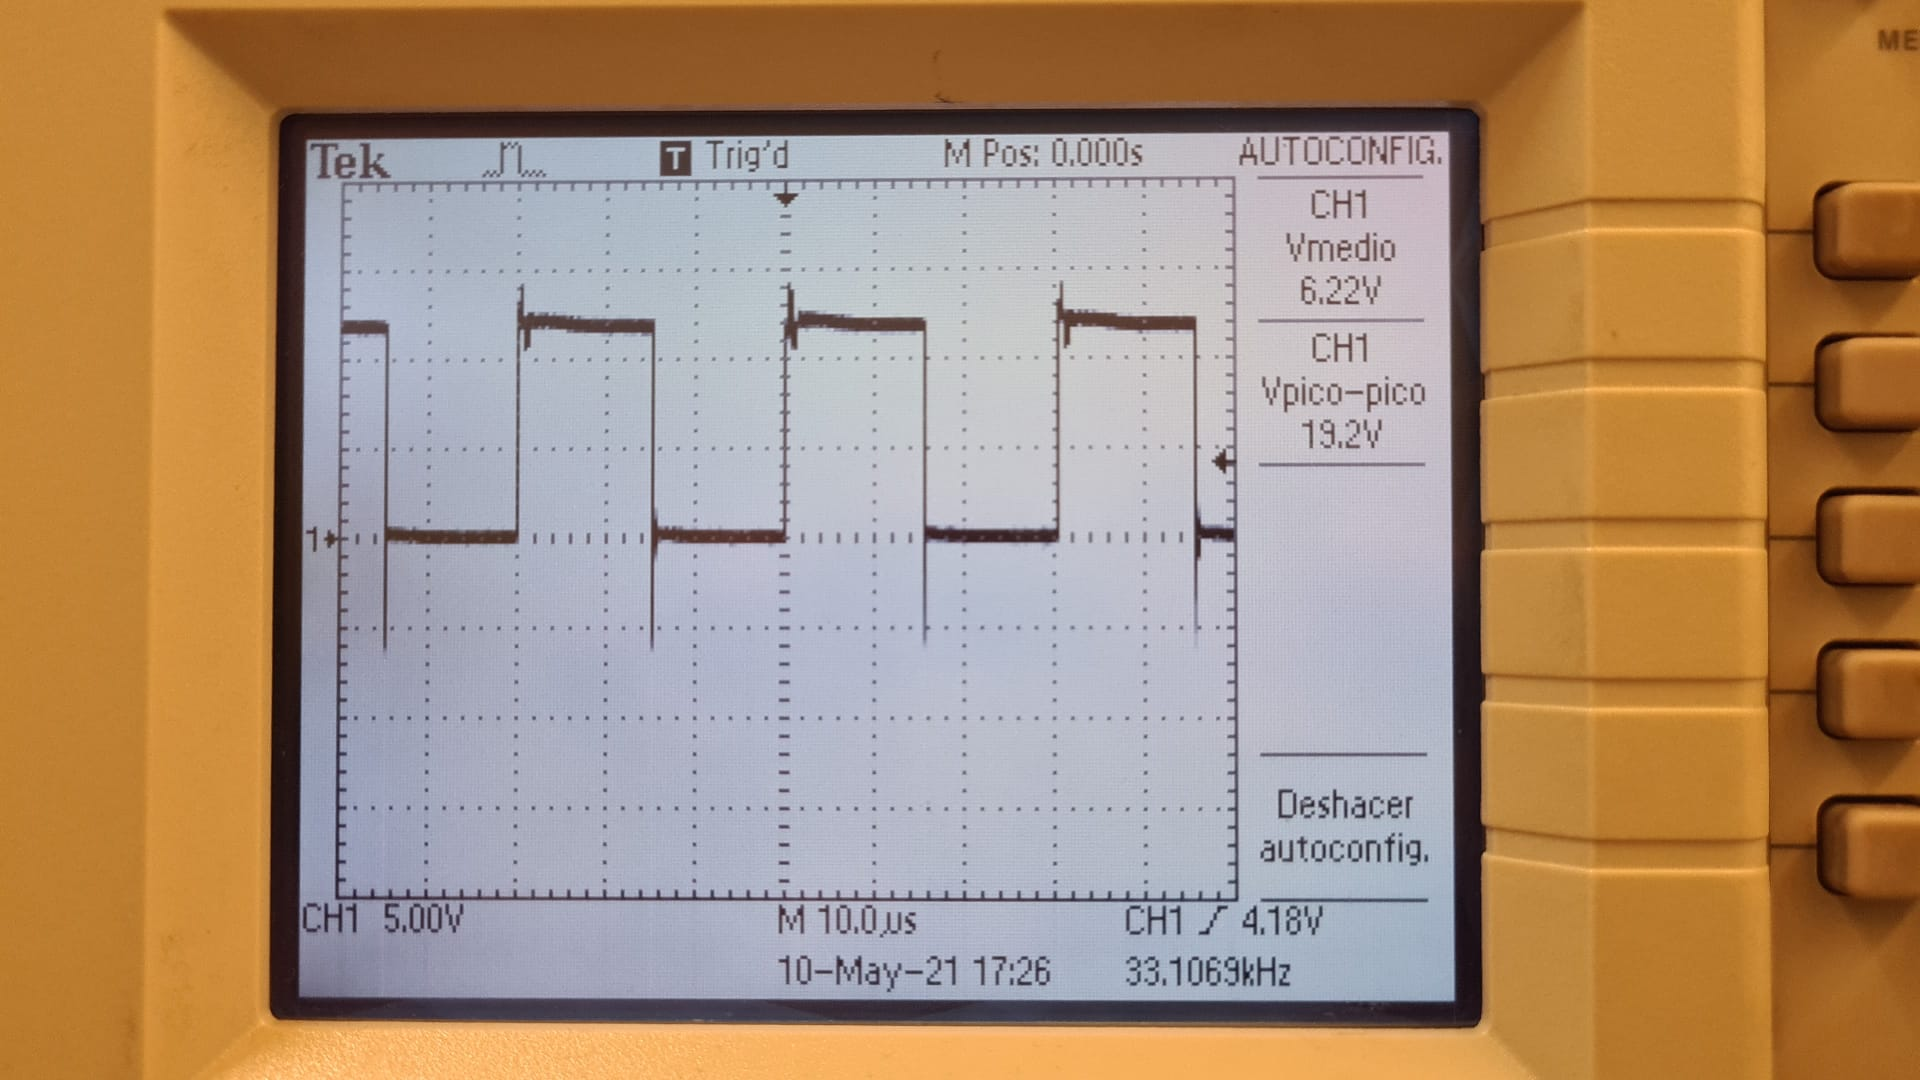
\includegraphics[width=80mm]{4_7_min.jpeg}
		\end{center}
	\end{figure}
	
	\textbf{Qüestió 2 i 3:} Quan ho posem a  $f = 40kHz$ tenim una amplitud al senyal de sortida de 12V. Te un cicle de treball $D = 0.5$, que es bastant bo per la practica.
	
	\textbf{Qüestió 4 i 5:} Podem veure aquí que tal i com esperavem el circuit nomes fa un puls. La tensió es de $12V$ i el temps es de $0.25ms$.
		
	\begin{figure}[H]
		\begin{center}
		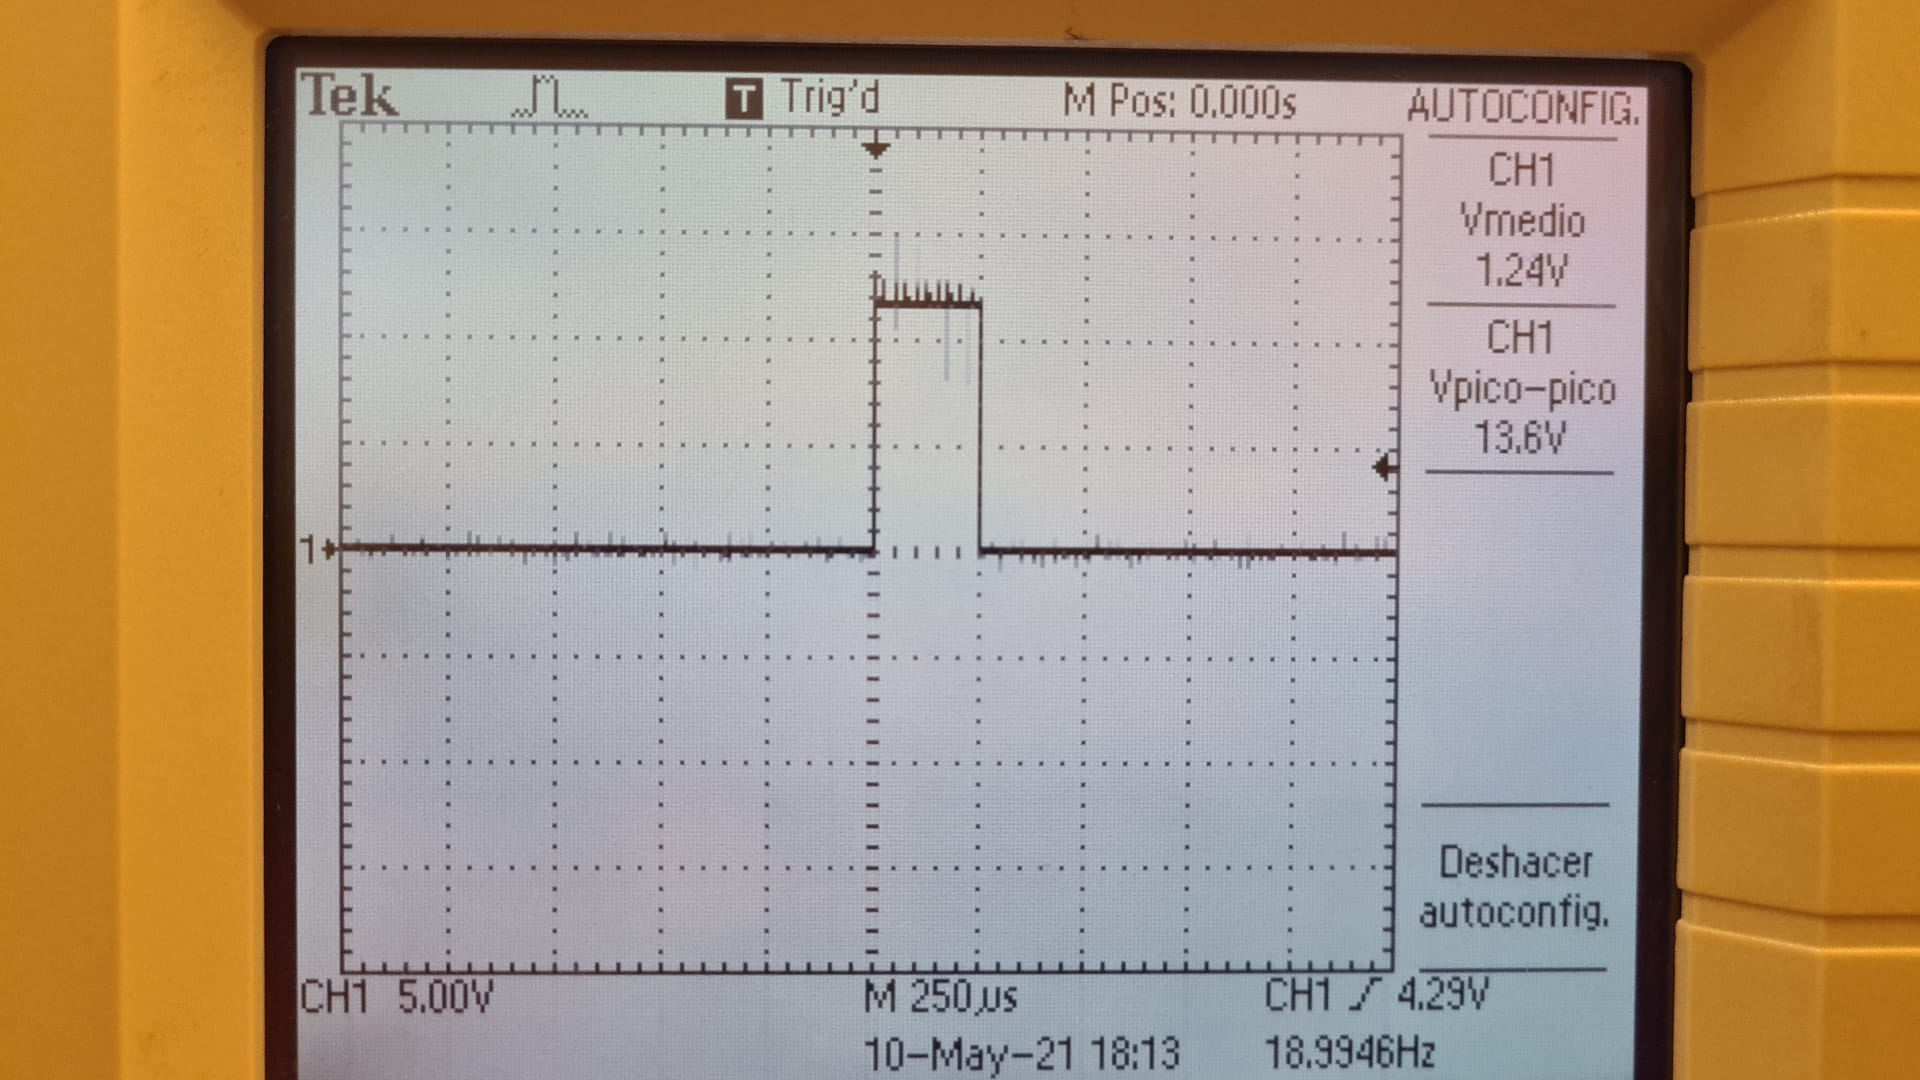
\includegraphics[width=80mm]{p4_4_2.jpeg}
		\end{center}
	\end{figure}
	
	\textbf{Qüestió 6:} Podem veure que tal i com haviem de fer hi han 10 polsos amb la frequencia de $40kHz$ de la sessió 1.
	
	\begin{figure}[H]
		\begin{center}
		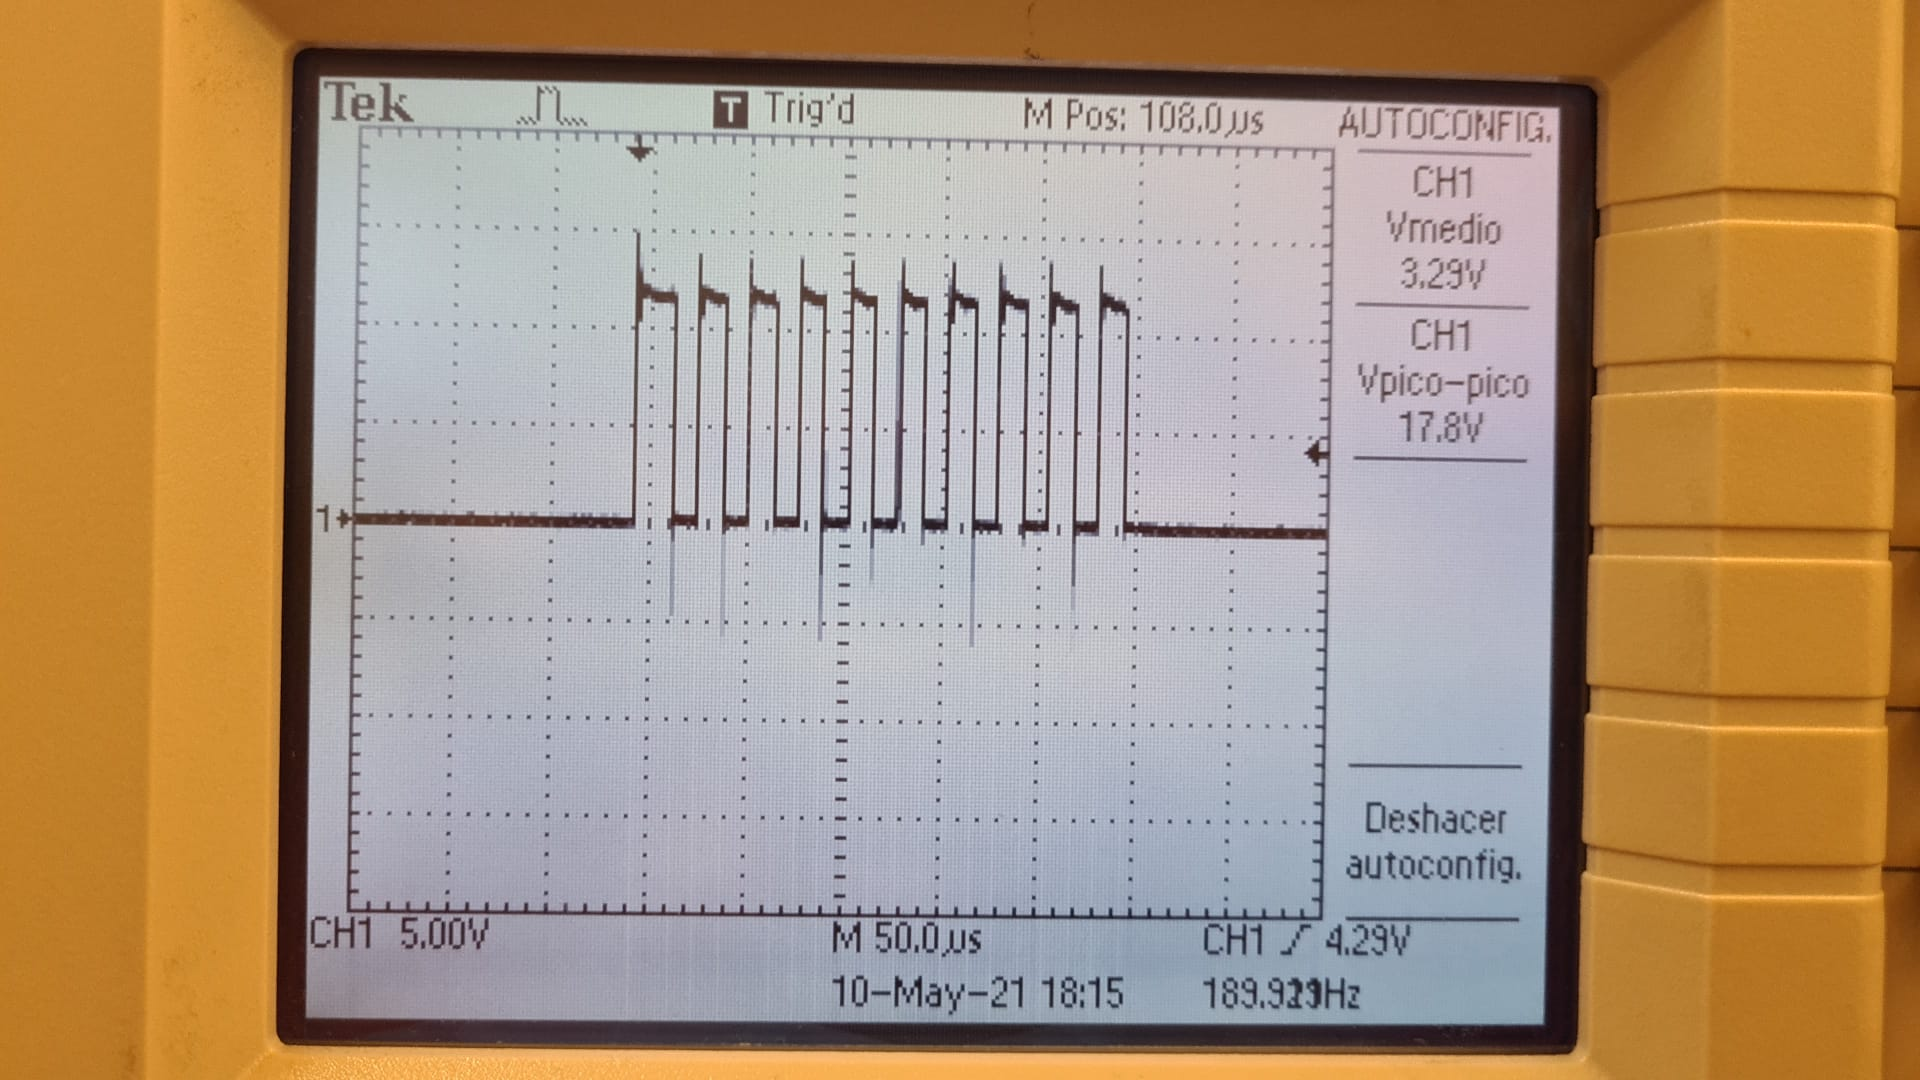
\includegraphics[width=80mm]{p4_8.jpeg}
		\end{center}
	\end{figure}
	
	\textbf{Qüestió 7:} A la primera fotografia podem veure el senyal a la sortida del receptor i a la segona a la sortida del amplificador. La amplitud despres del amplificador es de aproximadament $V = 1.8V$.
	
	\begin{figure}[H]
		\begin{center}
		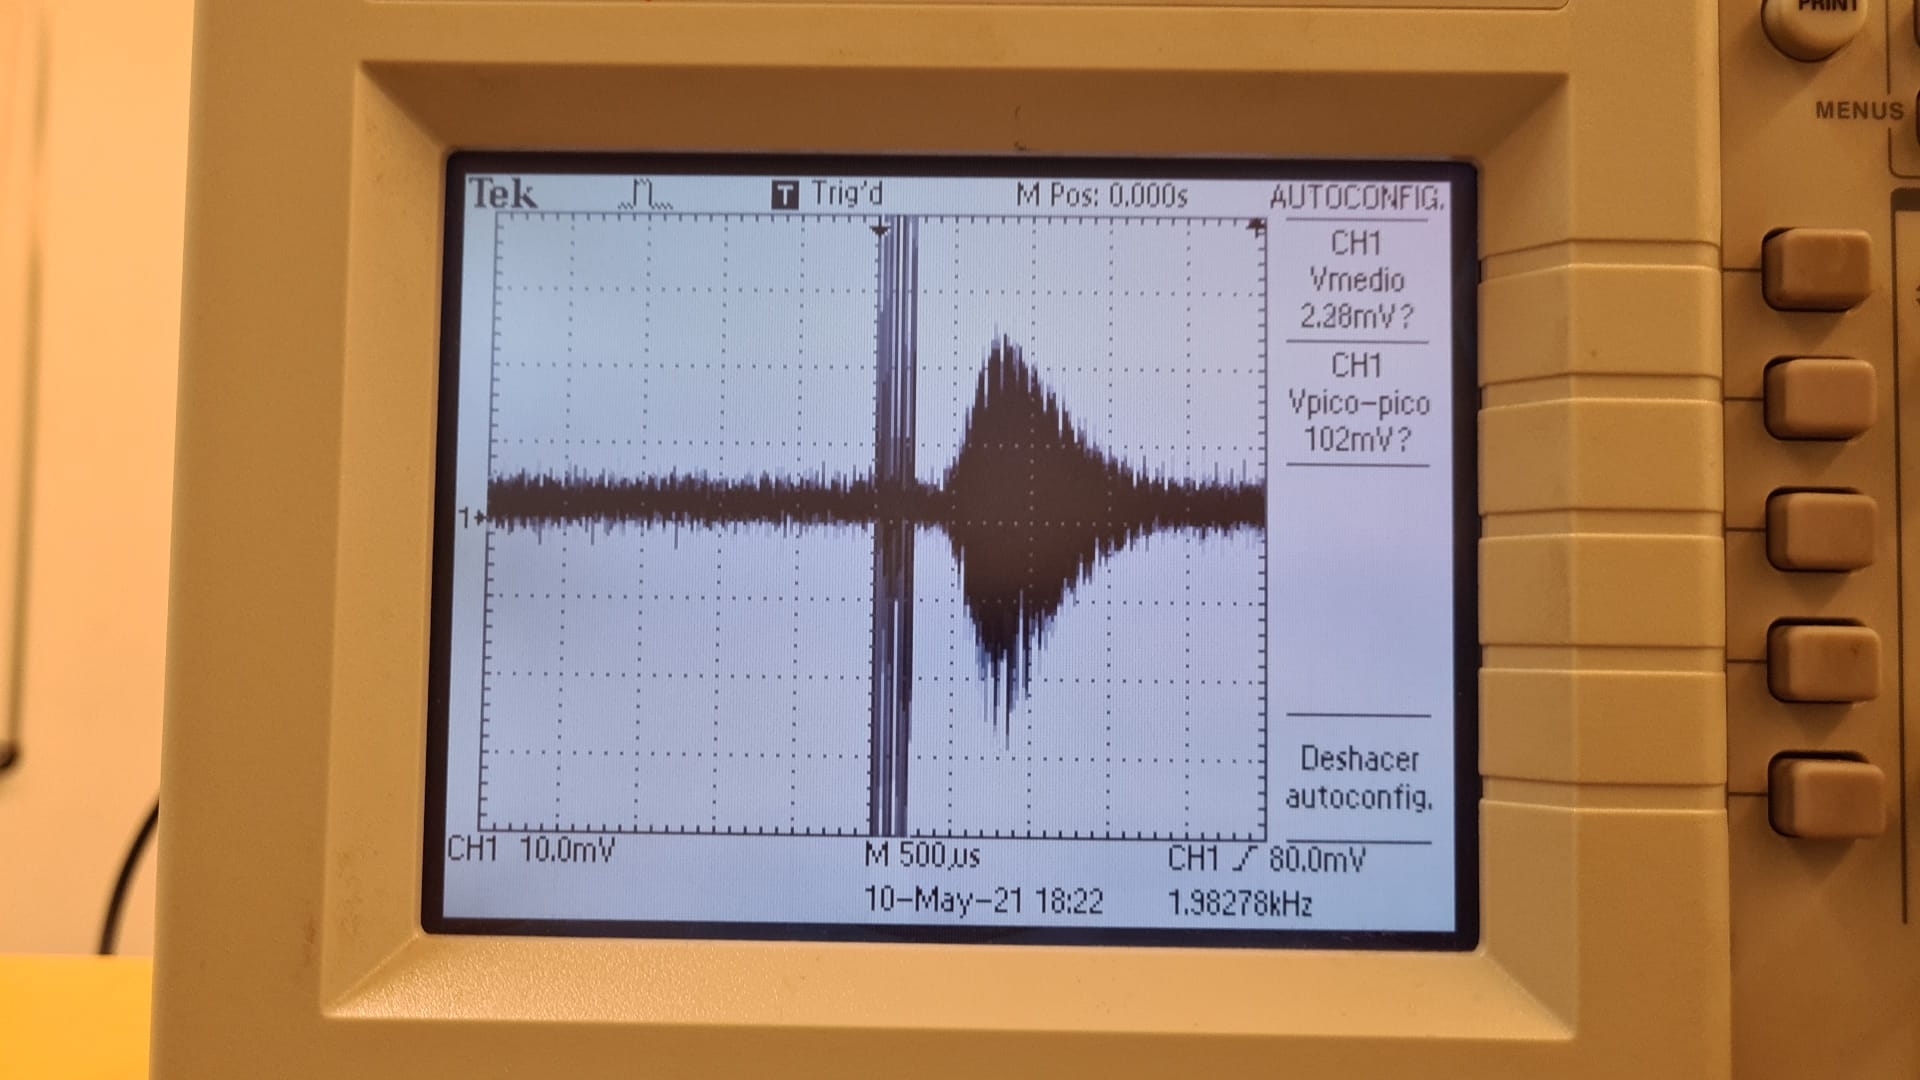
\includegraphics[width=80mm]{p4_9.jpeg}
		\end{center}
	\end{figure}
	
	\begin{figure}[H]
		\begin{center}
		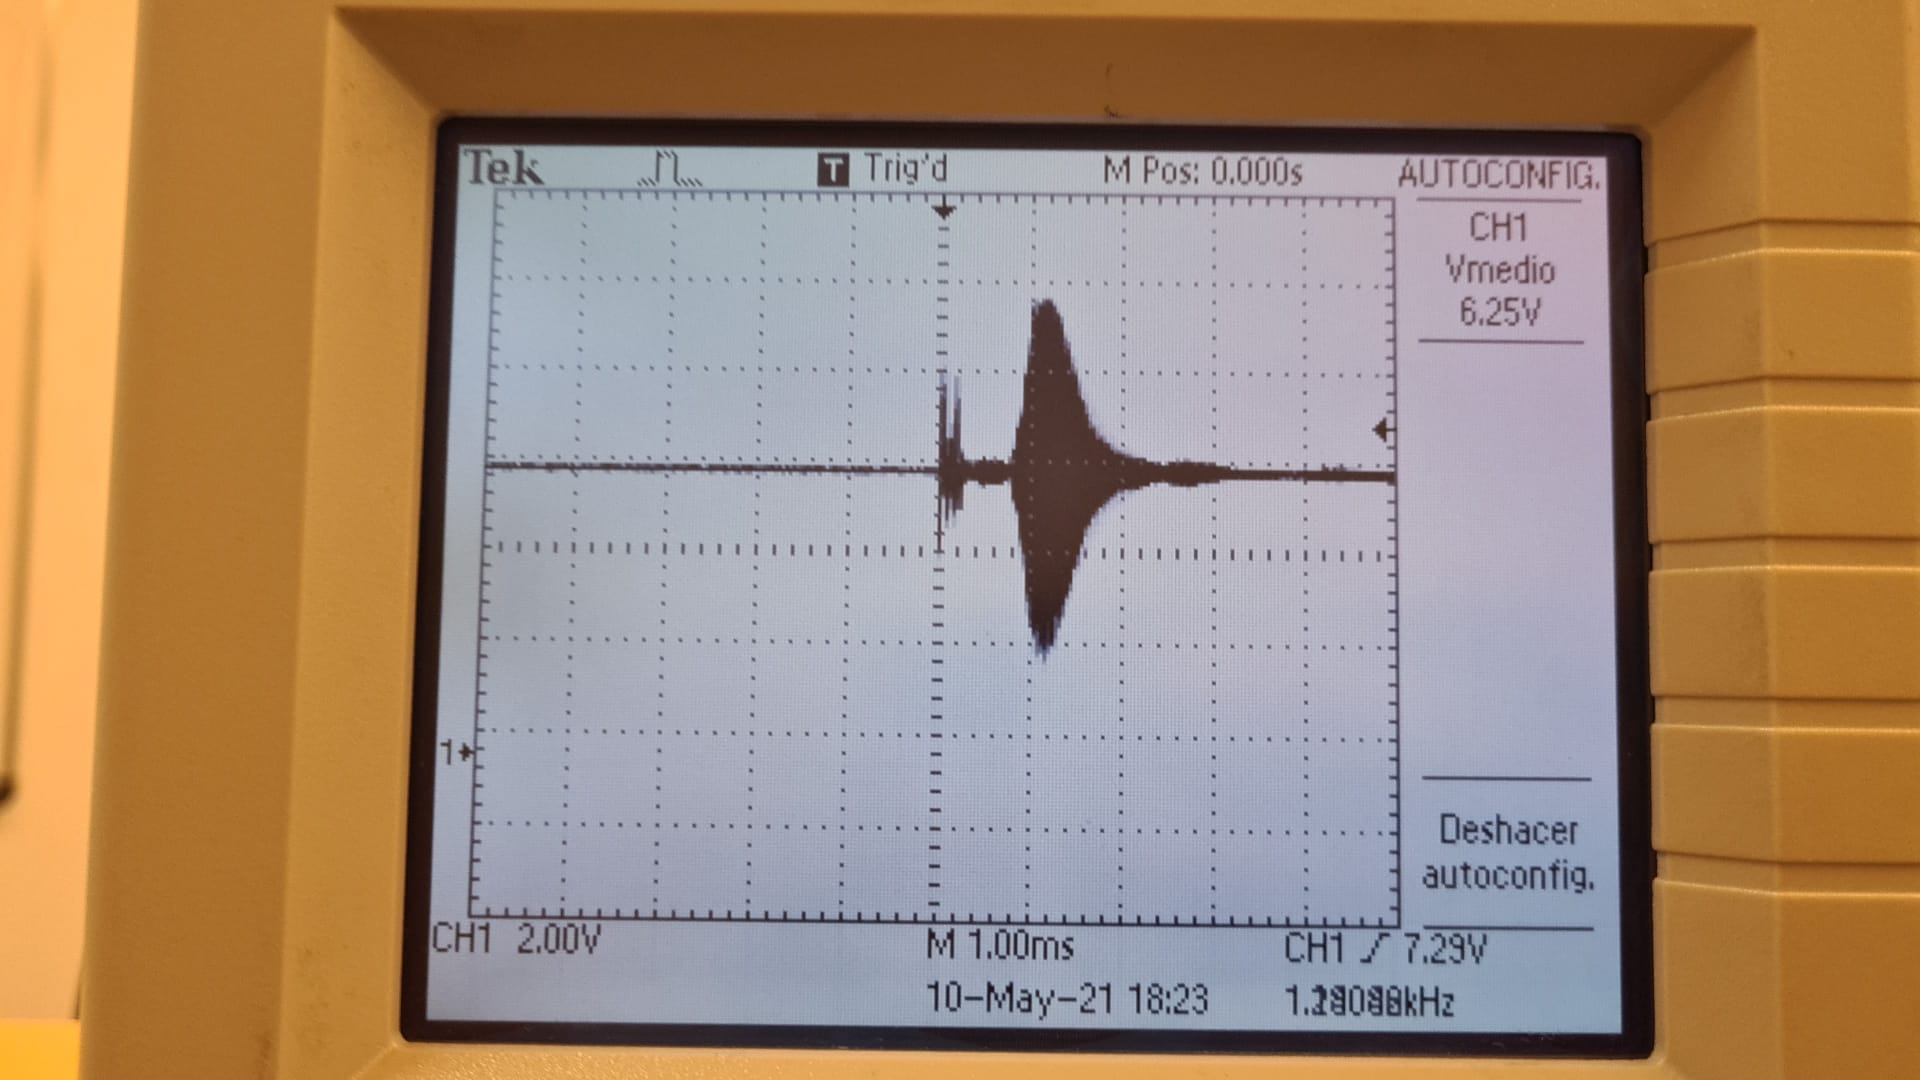
\includegraphics[width=80mm]{p4_10.jpeg}
		\end{center}
	\end{figure}
	
	\section{Sessió 3}
	
	Aquesta es la sessió mes curta de les 3.\\
	
	\textbf{Qüestió 1, 2 i 3:} Podem veure que la frequencia minima es de $f = 14.4kHz$ i màxima $f = 20.2kHz$. Les amplituds de les senyals son de $13V$. El cicle de treball per a $k = 17kHz$ es de $D = 0.4$.
	
	\begin{figure}[H]
		\begin{center}
		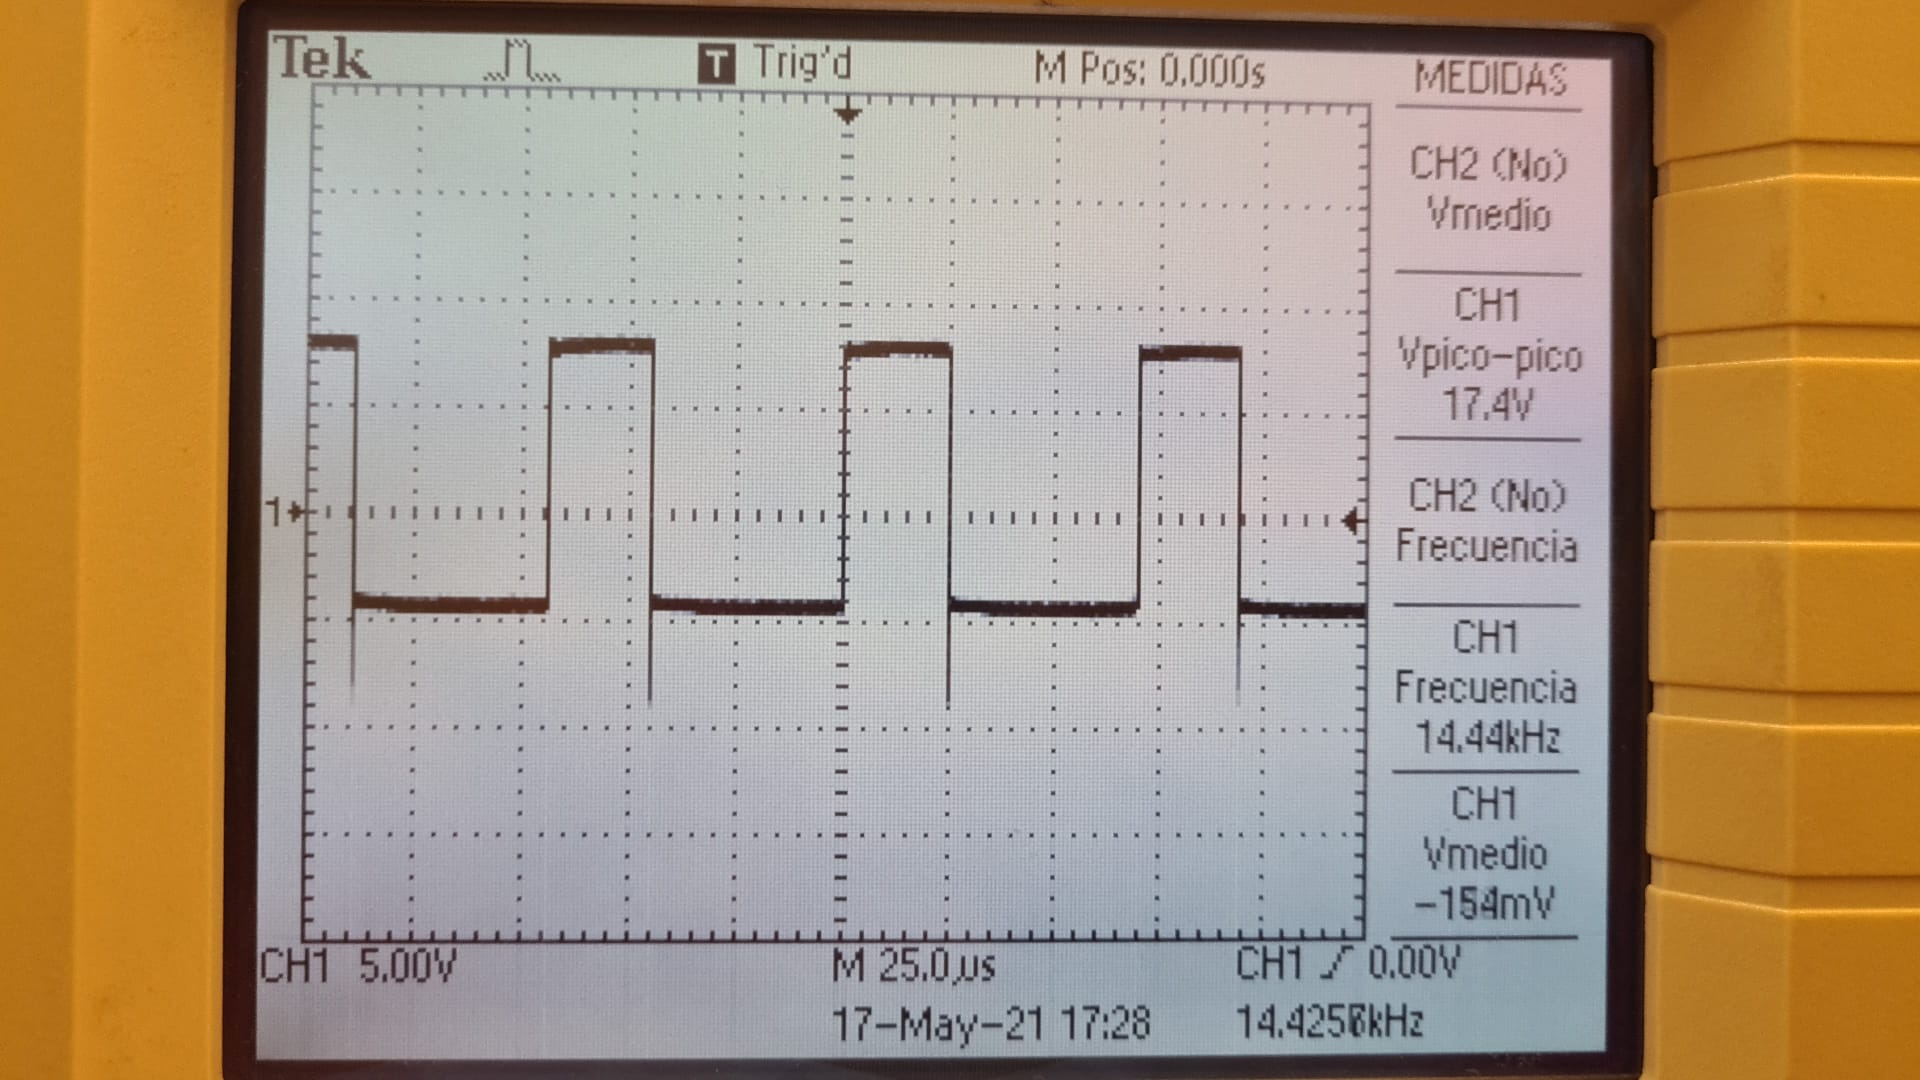
\includegraphics[width=80mm]{p4_11.jpeg}
		\end{center}
	\end{figure}
	
	\begin{figure}[H]
		\begin{center}
		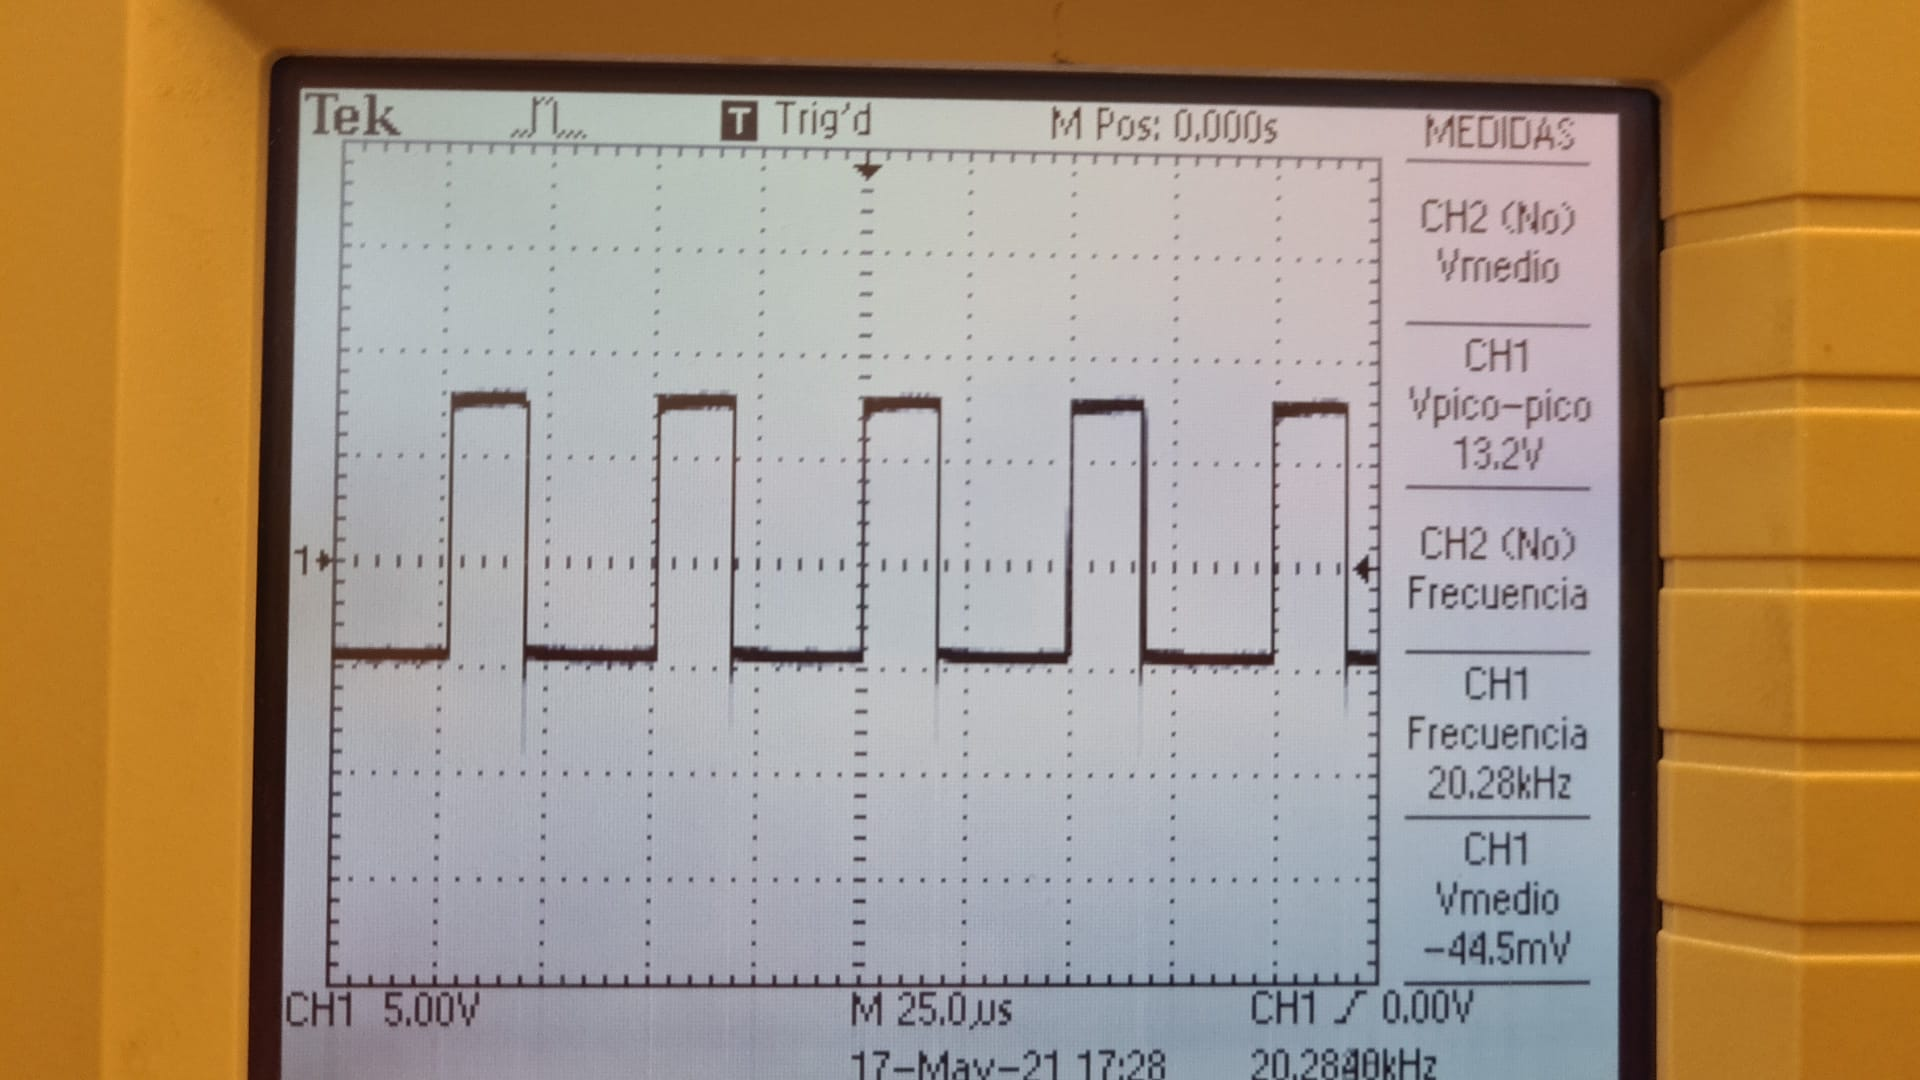
\includegraphics[width=80mm]{p4_12.jpeg}
		\end{center}
	\end{figure}
	
	\textbf{Qüestió 4} Veiem ara la senyal a la entrada del emisor i al final del circuit. Veiem que en funció de la distancia a la que esta l'objecte la separació entre els senyals augmenta o disminueix. Amb aquesta informació i la del rellotge de $17kHz$ creat a la questió 1 podem saber la distancia a la que es troba l'objecte.
	
	\begin{figure}[H]
		\begin{center}
		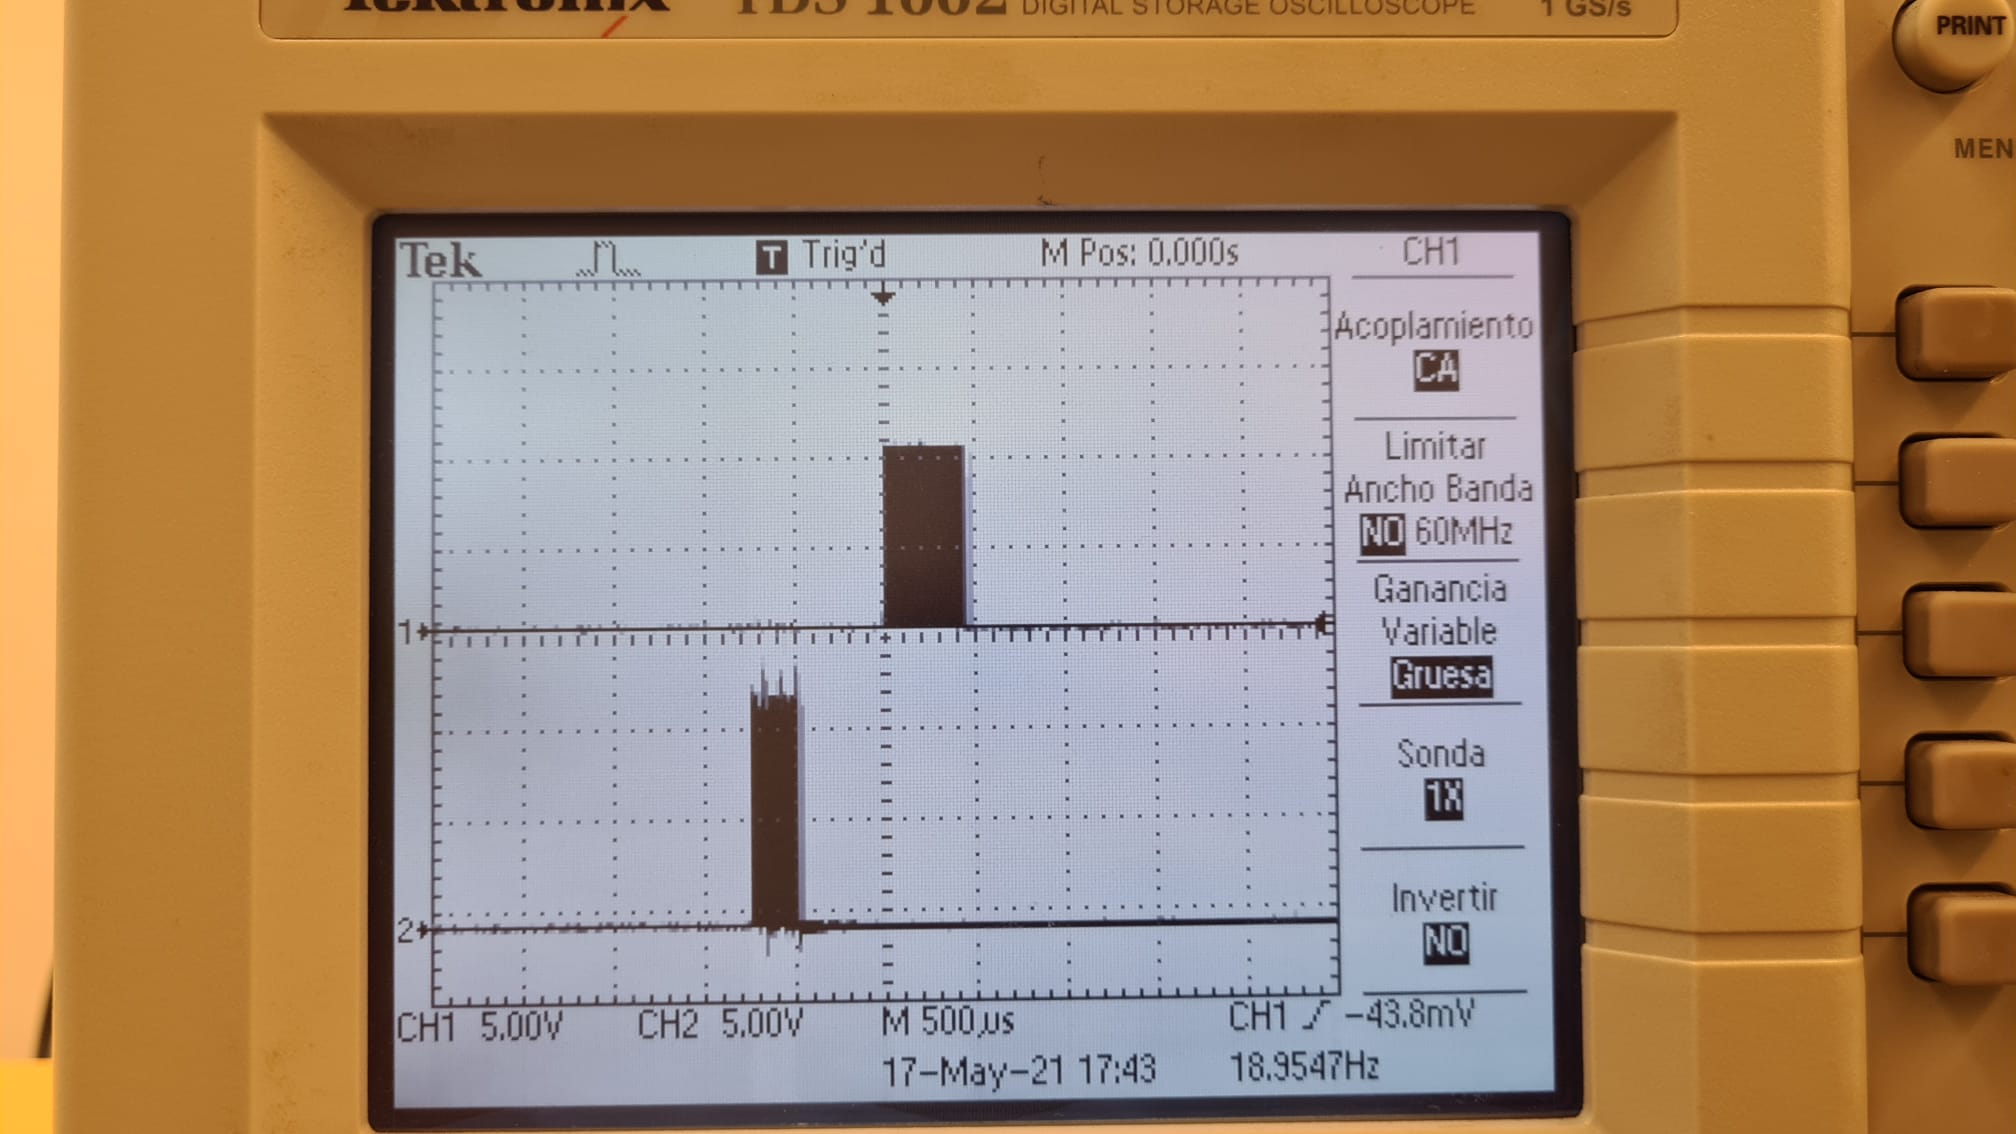
\includegraphics[width=80mm]{p4_13.jpeg}
		\end{center}
	\end{figure}
	
	\begin{figure}[H]
		\begin{center}
		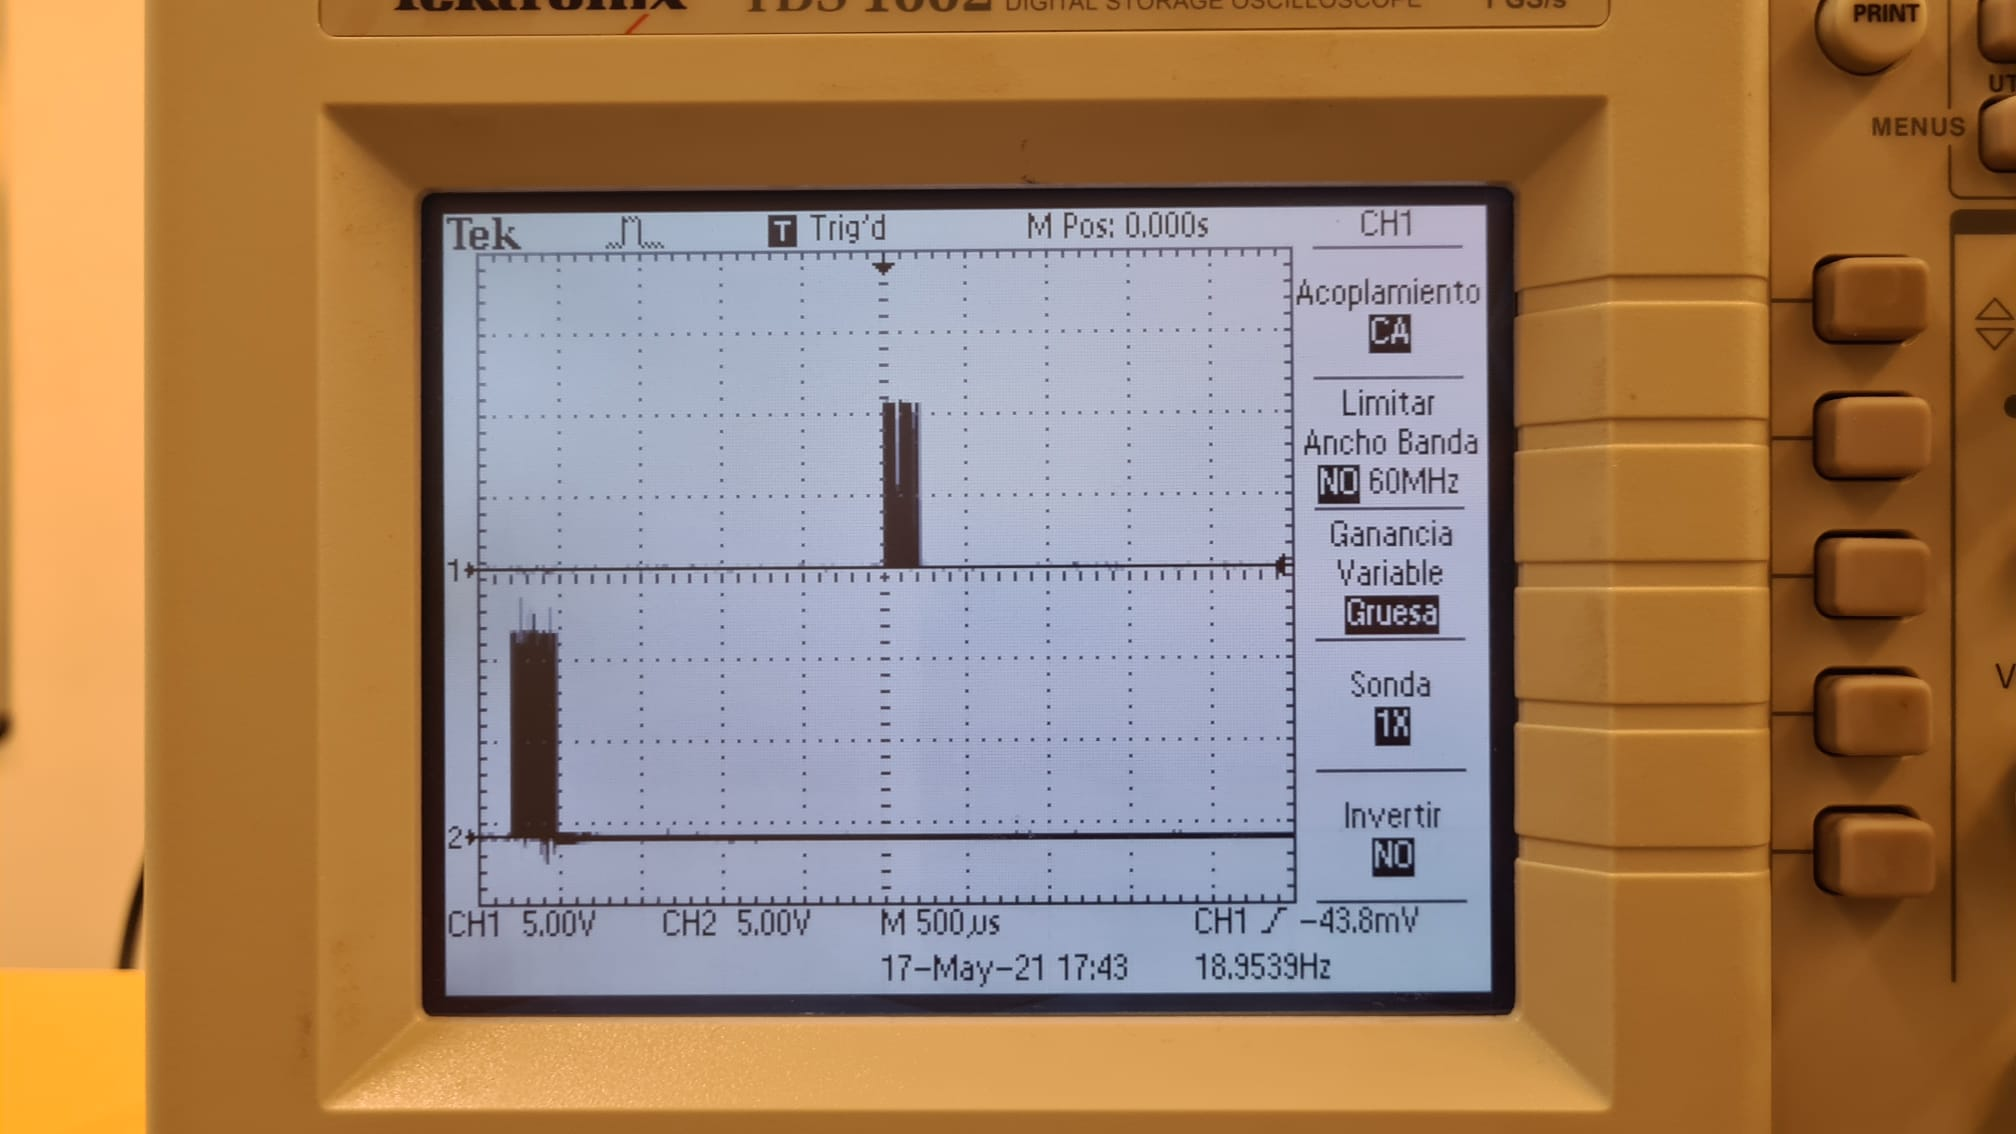
\includegraphics[width=80mm]{p4_14.jpeg}
		\end{center}
	\end{figure}
	
	\textbf{Qüestió 5} L'abast del nostre mesurador de distancia es de $62cm$ tal i com podem veure a la següent imatge. Veiem a la següent imatge el circuit complet.
	
	\begin{figure}[H]
		\begin{center}
		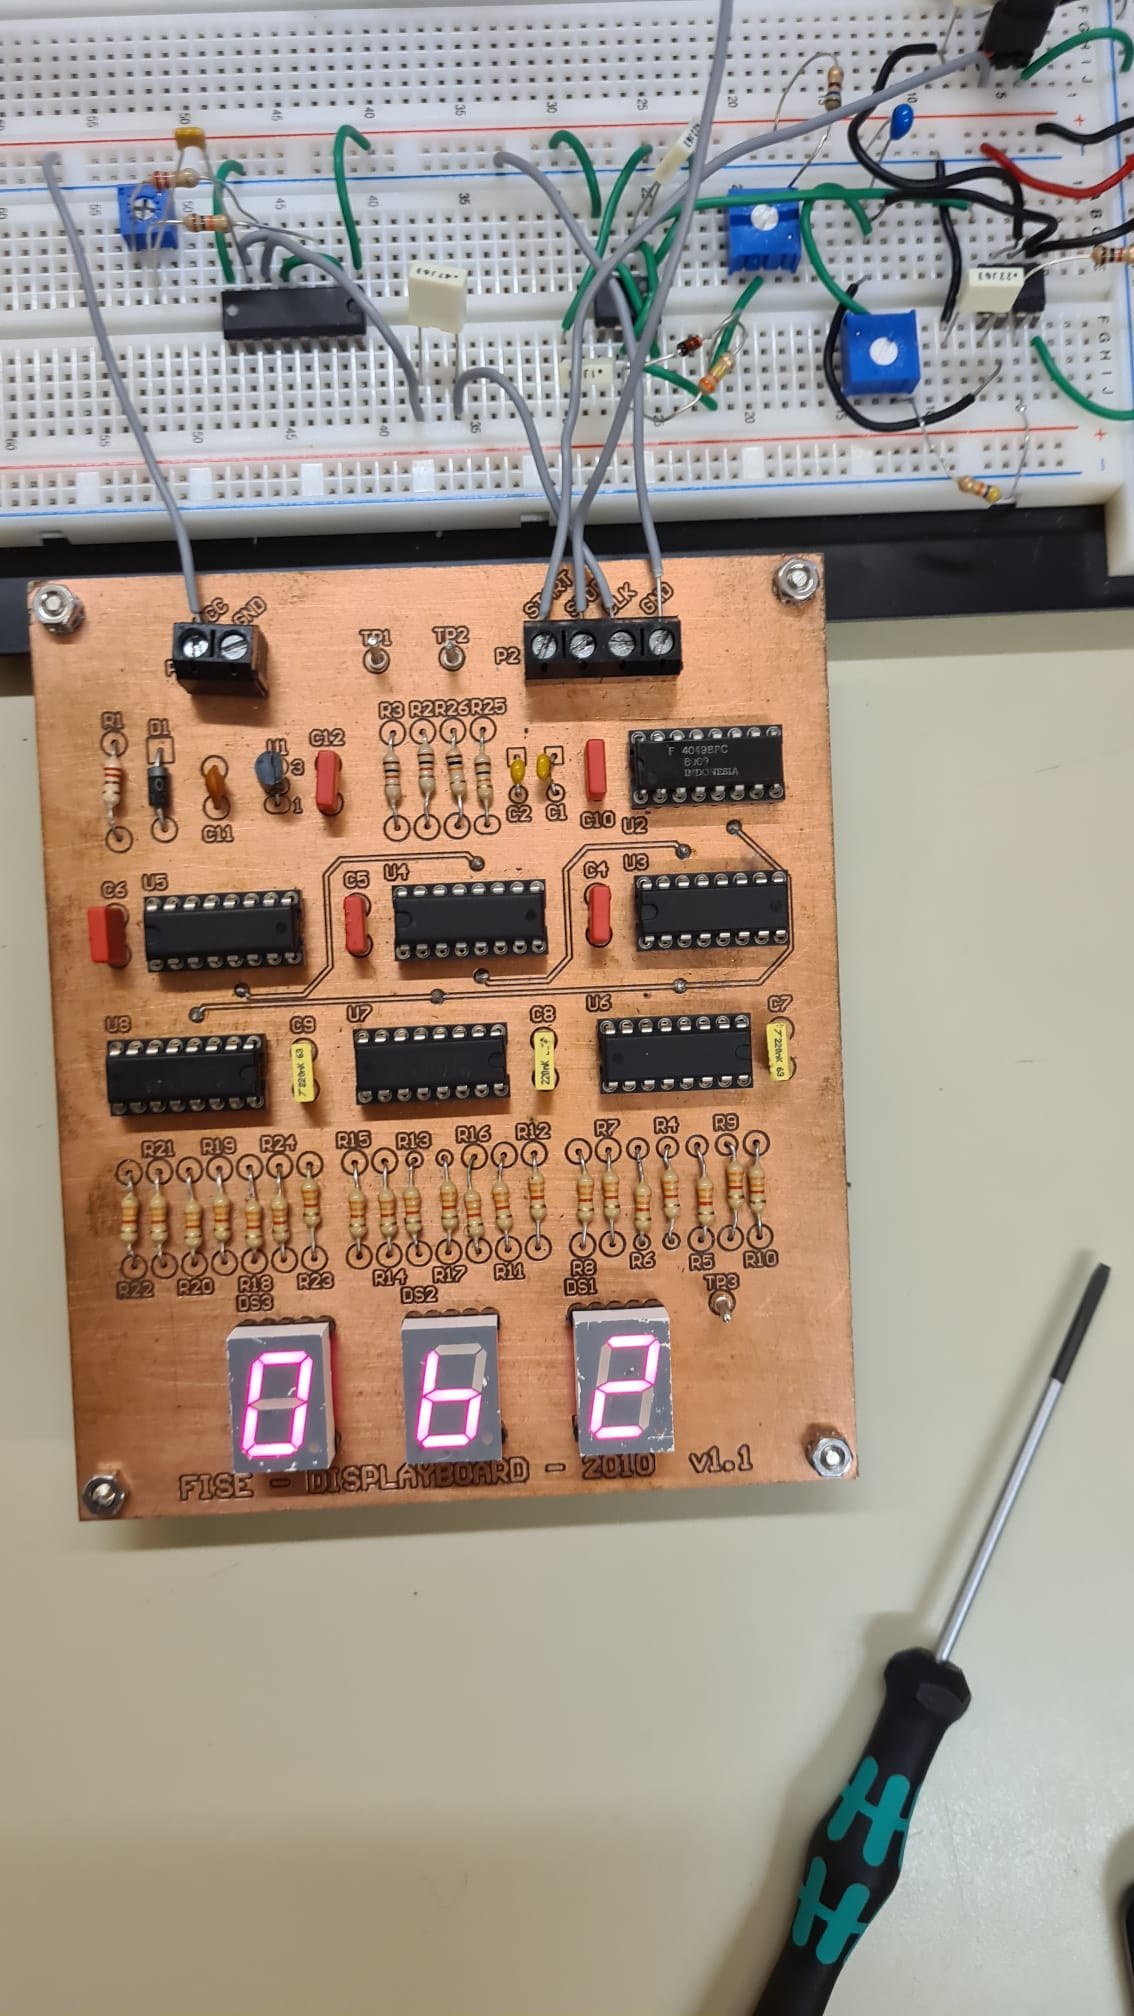
\includegraphics[width=80mm]{p4_15.jpeg}
		\end{center}
	\end{figure}
	
	\begin{figure}[H]
		\begin{center}
		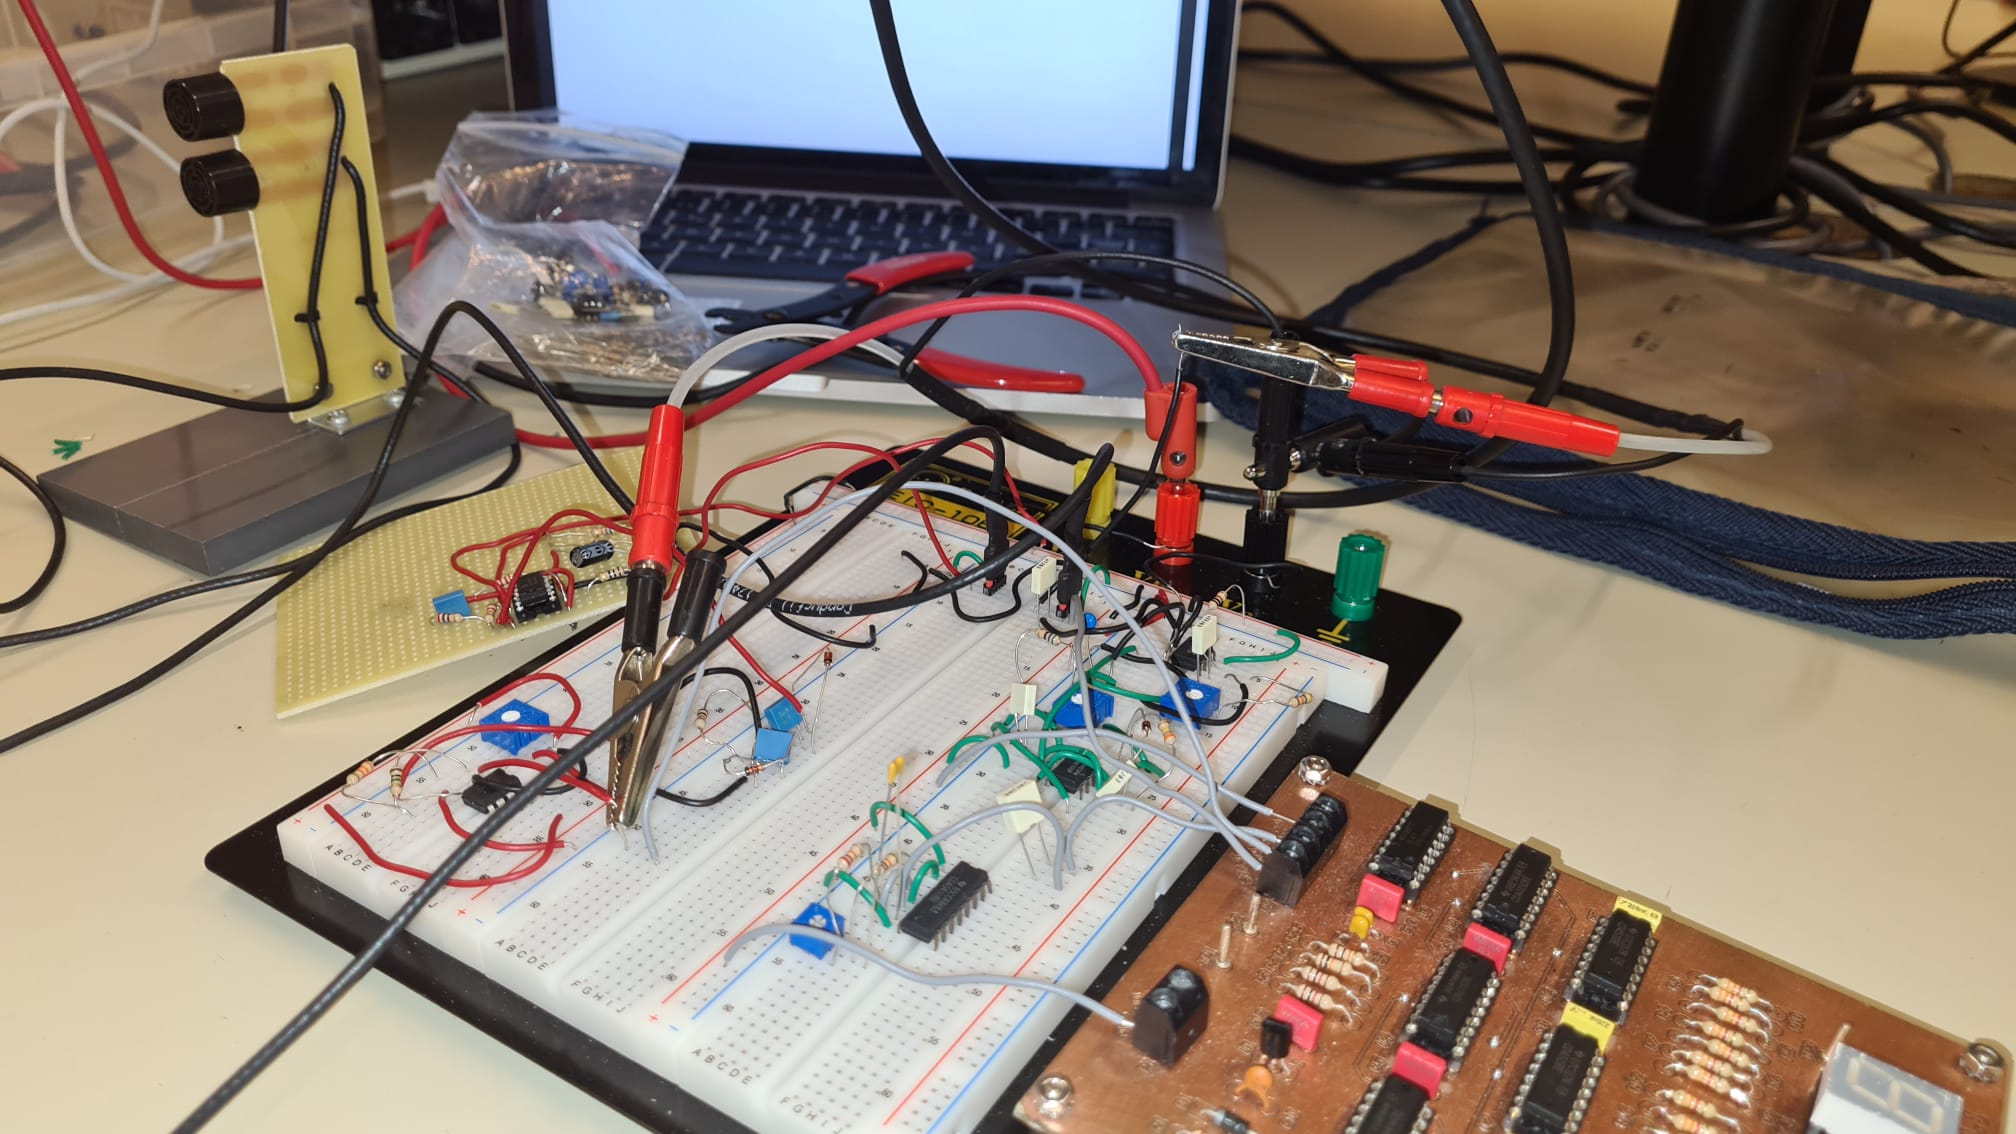
\includegraphics[width=120mm]{p4_16.jpeg}
		\end{center}
	\end{figure}
	
\end{document}










